% Created 2018-12-23 周日 18:27
\documentclass[a5paper,twoside]{book}
\usepackage[T1]{fontenc}
\usepackage{fixltx2e}
\usepackage{graphicx}
\usepackage{longtable}
\usepackage{float}
\usepackage{wrapfig}
\usepackage{rotating}
\usepackage[normalem]{ulem}
\usepackage{amsmath}
\usepackage{textcomp}
\usepackage{marvosym}
\usepackage{wasysym}
\usepackage{amssymb}
\usepackage[colorlinks]{hyperref}
\tolerance=1000
\usepackage{ctex}
\renewcommand{\contentsname}{目录}
\renewcommand{\figurename}{图}
\renewcommand{\tablename}{表}
\usepackage{geometry}
\usepackage{color}
\usepackage{listings}
\geometry{left=2cm,right=2cm,top=2cm,bottom=2cm}
\renewcommand{\maketitle}{%%%%%%%%%%%%%%%%%%%%%%%%%%%%%%%%%%%%%%%%%%%%%%%%%%%%%%%%%%%%%%%%%
% Contents: The title page
% $Id: title.tex,v 1.2 2003/03/19 20:57:47 oetiker Exp $
%%%%%%%%%%%%%%%%%%%%%%%%%%%%%%%%%%%%%%%%%%%%%%%%%%%%%%%%%%%%%%%%%
% 九皋兵法:wengchenyang@foxmail.com
%%%%%%%%%%%%%%%%%%%%%%%%%%%%%%%%%%%%%%%%%%%%%%%%%%%%%%%%%%%%%%%%%

\ifx\pdfoutput\undefined % We're not running pdftex
\else
%\pdfbookmark{Title Page}{title}
\pdfbookmark{标题页}{title}
\fi
\newlength{\centeroffset}
\setlength{\centeroffset}{-0.5\oddsidemargin}
\addtolength{\centeroffset}{0.5\evensidemargin}
%\addtolength{\textwidth}{-\centeroffset}
\thispagestyle{empty}
\vspace*{\stretch{1}}
\noindent\hspace*{\centeroffset}\makebox[0pt][l]{\begin{minipage}{\textwidth}
\flushright
{\huge \bfseries 御宇长策}
\noindent\rule[-1ex]{\textwidth}{5pt}\\[2.5ex]
\hfill\emph{\Large 车马冷招研究与赏析}
%{\Huge\bfseries The Not So Short\\
%Introduction to \LaTeXe
%
%}
%\noindent\rule[-1ex]{\textwidth}{5pt}\\[2.5ex]
%\hfill\emph{\Large Or \LaTeXe{} in \pageref{verylast} minutes}
\end{minipage}}

\vspace{\stretch{1}}
\noindent\hspace*{\centeroffset}\makebox[0pt][l]{\begin{minipage}{\textwidth}
\flushright
{\bfseries 作者:} 翁晨阳\\[1.5ex]
              上海核工程研究设计院象棋兴趣小组\\[1.5ex]
{\bfseries 版本:} Version~0.0, Dec 02, 2018\\[3ex]
%{\bfseries 中文翻译:} 中文~\TeX{}~学会\\[1.5ex]
%{\bfseries 中文版本:} 版本~4.20,二零零七年九月
\end{minipage}}


%\addtolength{\textwidth}{\centeroffset}
\vspace{\stretch{2}}


% \pagebreak
% \thispagestyle{empty}
% \begin{small}
% %  Copyright \copyright 1995-2005 Tobias Oetiker and Contributers.  All rights reserved.
  

%   This document is free; you can redistribute it and/or modify it
%   under the terms of the GNU General Public License as published by
%   the Free Software Foundation; either version 2 of the License, or
%   (at your option) any later version.
% %   这份文档是免费的;在~Free Software Foundation~颁布的~GNU~通用出版许可证的条款下,
% %   你可以再版或者修改它。许可证可以是第二版,或者任何后继版本(随你意)。

%   This document is distributed in the hope that it will be useful, but
%   WITHOUT ANY WARRANTY; without even the implied warranty of
%   MERCHANTABILITY or FITNESS FOR A PARTICULAR PURPOSE\@.  See the GNU
%   General Public License for more details.
% %   发布这份文档是希望它会有用,但并不提供任何保障;甚至没有用于商业的或者
% %   适用某一特定目的的暗含保证。更多的细节请查看~GNU~通用出版许可证。

%   You should have received a copy of the GNU General Public License
%   along with this document; if not, write to the Free Software
%   Foundation, Inc., 675 Mass Ave, Cambridge, MA 02139, USA.
% %   你应该随这份文档收到一份~GNU~通用出版许可证的拷贝;如果没有,写信到
% %   ~Free Software Foundation,地址:675 Mass Ave, Cambridge, MA 02139, USA。

% \end{small}


% \endinput

%

% Local Variables:
% TeX-master: "lshort2e"
% mode: latex
% mode: flyspell
% End:
}
\usepackage{paralist}
\usepackage{cchess}
\setcounter{secnumdepth}{4}
\author{上海核工程研究设计院象棋兴趣小组}
\date{\textit{<2018-12-02 周一>}}
\title{御宇长策}
\hypersetup{
  pdfkeywords={},
  pdfsubject={},
  pdfcreator={Emacs 25.3.1 (Org mode 8.2.10)}}
\begin{document}

\maketitle
\renewcommand{\contentsname}{目录}
\renewcommand\listfigurename{插\ 图\ 目\ 录}
\frontmatter
\chapter*{前言}

车主势,纵横;马主变,制奇。

当对方将位不安、士象不整或者防守子力薄弱时,车马常常能
发起奇袭,古籍中谓之“车马冷招”,这四个字充分体现了车
马配合战术打击的突然性。

车马的突袭之所以可得此美名,原
因大概在于车马这两种子力是天然的进攻拍档。到了残局阶段,盘面
子力减少,空间开阔,为车马威力的发挥创造了条件。车走直
线可纵横如电,寒
气森森,而马走曲线可回环奔跃,威震八面,车马两枚子之间
就可以自然而言形成纵横两路的立体攻势。与之相对的是车需
与天炮和地炮两门重炮才能形成立体攻势。

而且车马之间的配合方式是多姿多彩的,可以组成多种催杀的阵形,如卧槽马、钓鱼
马、高钓马、八角马、高位花心马、低位花心马、篡位马、花
心车等,本书中将车马之间这些基本的催杀阵形一一举例进行
介绍。

在掌握以上基本的攻击阵形的基础上,还需要掌握如何
依据局面在各种催杀阵形之间切换,由于将帅只能在九宫内行
走,而且每次只能走一步,这些都为持车马进攻的一方提供了变换阵
型进攻的诸多可能性,常见的手段包括:马限制将位后车的打将顿挫、
车帅限制黑将活动空间后的绕圈马连续将军同时实现马的大范围转移、拔簧马闪
击变换车位、前马后车阵型借车力变换马位等,而且变换阵型的过程
中常可以顺手牵羊消除黑方的防御力量,
这也是车马冷招令人防不胜防的另一原因。本书中也将针对如
何在各种催杀阵形之间进行切换这一主题举例说明。

准备好了吗?让我们一起来领略车马冷着之美!



\tableofcontents
\listoffigures
\mainmatter
\setlength{\parskip}{1em}

\let\itemize\compactitem
\let\enditemize\endcompactitem
\let\enumerate\compactenum
\let\endenumerate\endcompactenum
\let\description\compactdesc
\let\enddescription\endcompactdesc
\chapter{术语}
\label{sec-1}
\begin{description}
\item[{卧槽马}] 位于对方下二路与三路线或七路线交点的马。
\item[{钓鱼马}] 位于对方布置线与三路线或七路线交点的马。
\item[{高钓马}] 位于对方卒林线与三路线或七路线交点的马。
\item[{高位花心马}] 位于对方3卒和中卒之间的马,或者位于对方
7卒与中卒之间的马。
\item[{低位花心马}] 位于对方底象位的马。
\item[{炮位马}] 位于对方炮台位的马。
\item[{篡位马}] 位于对方将位的马。
\item[{虎穴马}] 位于对方底线士位的马。
\item[{八角马 }] 位于对方高士角位的马。
\item[{象腰马 }] 位于对方九宫内象眼位的马。
\item[{侧锋马}] 位于对方下二路与二路线或八路线交点的马。
\item[{前锋马}] 位于对方沿河线和中路交叉点的马。
\item[{布置线}] 也称宫顶线,指经过九宫顶的横线。
\item[{天马}] 位于对方沿河线与肋道交点的马。
\end{description}

\chapter{卧槽马}
\label{sec-2}

\section{卧槽马基础型}
\label{sec-2-1}
\begin{figure}[H]
\centering
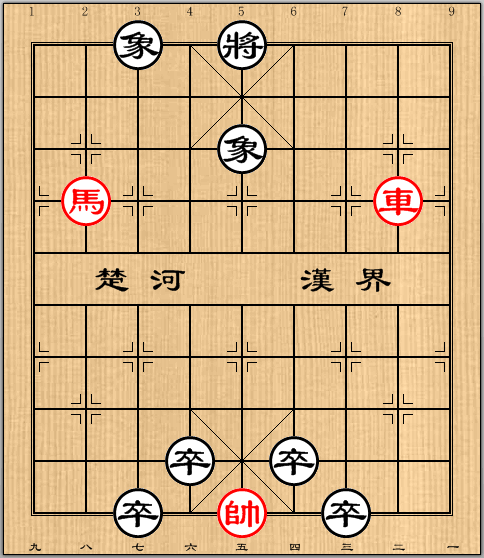
\includegraphics[width=5cm]{pic/卧槽马-基础型.png}
\caption{卧槽马-基础型}
\end{figure}


如图所示为卧槽马的基础型,当红车处于高位时,卧槽马可以
直接做杀:
\begin{itemize}
\item 黑方如果出将,红方可以平车将;
\item 黑方如果进将,红方可以进车将。
\end{itemize}


可见, \textbf{卧槽马和高车分居两翼时,对处于原位的将有很
强的杀伤力。}

\section{卧槽马-红方正确的一手是什么}
\label{sec-2-2}
\begin{figure}[H]
\centering
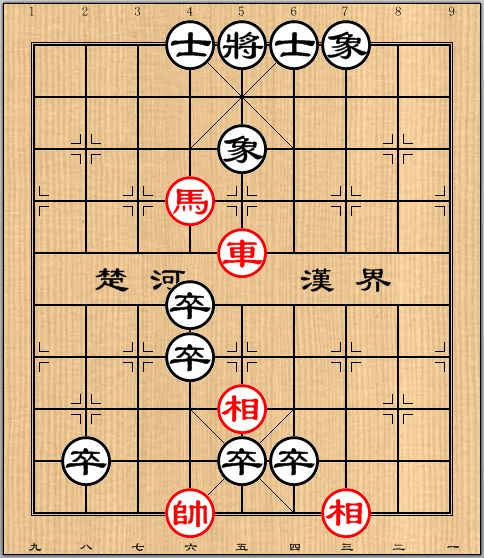
\includegraphics[width=5cm]{pic/卧槽马-红方正确的一手是什么.png}
\caption{卧槽马-红方正确的一手是什么}
\end{figure}


在这个局面下,马可以卧槽,可以挂角。而车马进攻常见的步骤也是
先用马将,把对方的老将从将位逼出来,使其处于受攻击的状态,利
用车马的联攻迫使黑将的位置越走越差,直至最终将杀。
但是这一局
无论是卧槽马将还是挂角马将,都没有能隔步成杀的手段。

但只要和\ref{sec-2-1}中的棋形进行对比,答案就是显而易见的,主
要的区别就是本局中的车位稍差,仅可以纵向打将,不可以横向打将,
所以红方只要把车走到一个更好的位置就可以了。

红方此时
正确的招法应该是 \textbf{车五平二} ,拉开车到红马即将奔赴的卧槽位的另一
侧,以下就可以确保以卧槽马成杀:
\begin{itemize}
\item 黑方如果置之不理,红方可以马六进七,将5进1,车二进三杀;
\item 黑方如果补士,红方可以马卧槽将再平肋车杀。
\end{itemize}

这个例子再次说明了 \textbf{卧槽马和高车分居两翼时对处于原
位的将有很强的杀伤力} 。

\section{卧槽马-弃车改变黑方的将门}
\label{sec-2-3}
\begin{figure}[H]
\centering
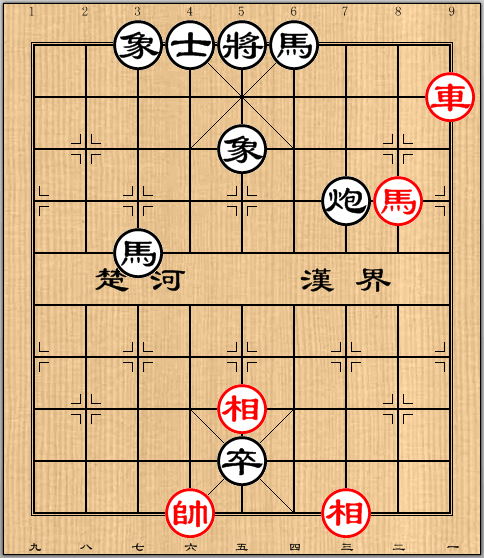
\includegraphics[width=5cm]{pic/卧槽马-弃车改变黑方的将门.png}
\caption{卧槽马-弃车改变黑方的将门}
\end{figure}

这一局红方的车位也不甚理想,不仅没有处于高位,而且还与卧槽马
处于同一翼。不过黑方的一匹马处于九宫内的士角位,这个弱点可以
被利用。红方可以弃车改变黑方的将门,再通过卧槽
马做杀。招法如下:

\begin{verbatim}
1. 马二进三,将5进1
2. 马三退四,将5退1
3. 车一平五!,将4平5
4. 马四进三。红胜。
\end{verbatim}

弃车改变将门或者封锁将路是一种常见的手段,在后面的钓鱼马和高
钓马中也可以看到类似的棋例。

\section{卧槽马-弃车改变黑方的将门位置又一例}
\label{sec-2-4}
这一局中,红车的位置更加糟糕,主要体现在以下几点:
\begin{itemize}
\item 处于低位
\item 和卧槽马处于同一翼
\item 处于卧槽马位,妨碍了卧槽马发挥威力
\end{itemize}


不过此局黑车居于九宫内的士角位,堵塞将路,同样可以被利用。红
方可以弃车砍中士做杀。弃车起了两个作用:
\begin{itemize}
\item 调整了黑方的将门的位置;
\item 腾出了卧槽马的马位。
\end{itemize}


\begin{figure}[H]
\centering
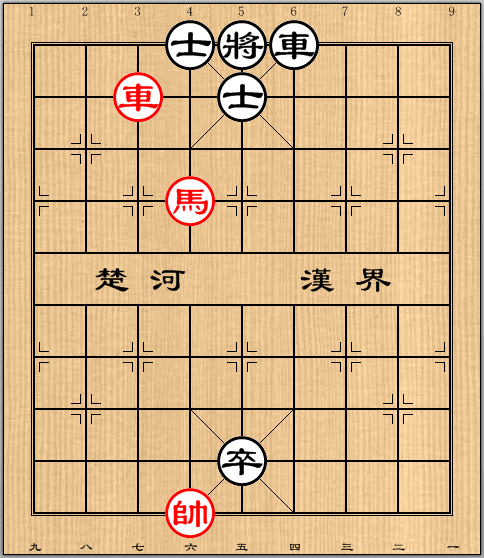
\includegraphics[width=5cm]{pic/卧槽马-弃车改变黑方的将门位置又一例.png}
\caption{卧槽马-弃车改变黑方的将门位置又一例}
\end{figure}

\begin{verbatim}
1. 车七平五!,士4进5
2. 马六进七。红胜。
\end{verbatim}

\section{卧槽马-借帅力拔簧杀}
\label{sec-2-5}

在\texttt{卧槽马基础型}中,红方的高车必须和卧槽马分居两翼,而当红车得
帅力助攻时,处于与卧槽马同一翼的肋道上也可以连杀。

如下图所示的局面,红马卧槽将之后黑方必须上将,红车可借帅力点
到下二路象腰位置,黑方必须下将,然后红方车四平六即可成杀,这
是卧槽马配合肋线上的车帅的一种常见的杀型。

所以通过这一局需要记住的就是, \textbf{肋线上的高车可以借帅力时,即使与卧槽马处于同一翼,
也有连杀的手段。}

\begin{figure}[H]
\centering
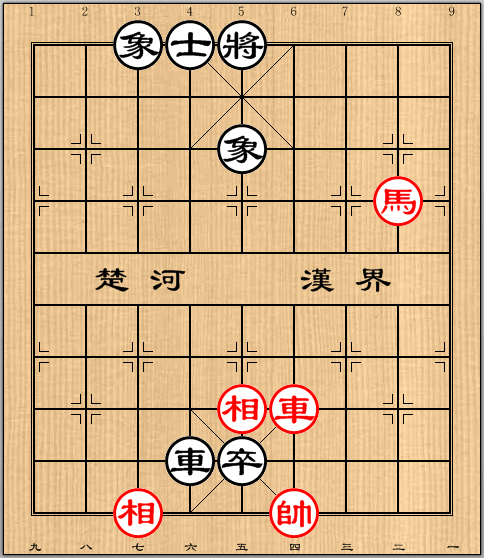
\includegraphics[width=5cm]{pic/卧槽马-借帅力拔簧杀.png}
\caption{卧槽马-借帅力拔簧杀}
\end{figure}

\begin{verbatim}
1. 马二进三,将5进1
2. 车四进六,将5退1
3. 车四平六。红胜
\end{verbatim}


\chapter{钓鱼马}
\label{sec-3}

\section{钓鱼马基础型}
\label{sec-3-1}
\begin{figure}[H]
\centering
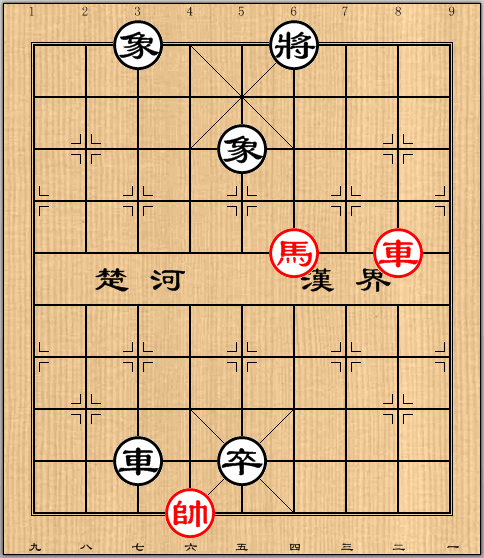
\includegraphics[width=5cm]{pic/钓鱼马-基础型.png}
\caption{钓鱼马基础型}
\end{figure}


如图所示的棋形中,红方马四进三后,黑方有上将和进将两种
选择,如果但由于钓鱼马正好控制了花心位,所以无论黑方上
将还是进将,红车都可以完成将杀:
\begin{itemize}
\item 黑方如果将6平5,红方可以车二进四杀。
\item 黑方如果将6进1,红方可以车二平四杀。
\end{itemize}


关于钓鱼马基础型,需要记住的是, \textbf{当黑方光将处于底线士
角位钓鱼马的马脚上,红方的钓鱼马配合高车,可以连杀。}

同时需要注意的是,所谓 \textbf{高车} , 简单来说是指车位高,
但更为切中要害的是提法是指 \textbf{可以纵横两向打将} 的车。
在上图所示的棋形中,如果黑方的3路底象换到了7路,那
么红方的车就无法车二进四到底线打将,这个时候红方的
车虽然仍然处于高位,但是已经不是一个严格意义的高车
了,或者说黑方的连环象发挥防守力,限制了红方“高
车”的威力。

\section{如何构造钓鱼马杀型}
\label{sec-3-2}
\subsection{如何构造钓鱼马杀型-例1}
\label{sec-3-2-1}

\begin{figure}[H]
\centering
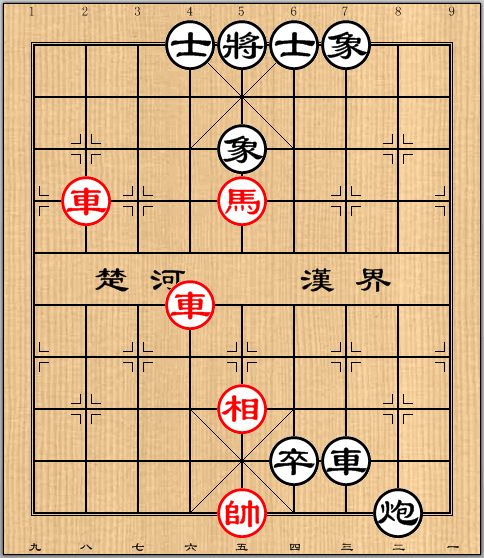
\includegraphics[width=5cm]{pic/钓鱼马-如何构造钓鱼马杀型.png}
\caption{钓鱼马-如何构造钓鱼马杀型}
\end{figure}

只要和\texttt{钓鱼马基础型}进行对比,这一局的答案就是显而易见的。红方
可以直接车六进五砍底士。

\begin{verbatim}
1. 车六进五!,将5平4
2. 马五进七,将4平5
3. 车八进三。红胜。
\end{verbatim}


\subsection{如何构造钓鱼马杀型-例2}
\label{sec-3-2-2}

\begin{figure}[H]
\centering
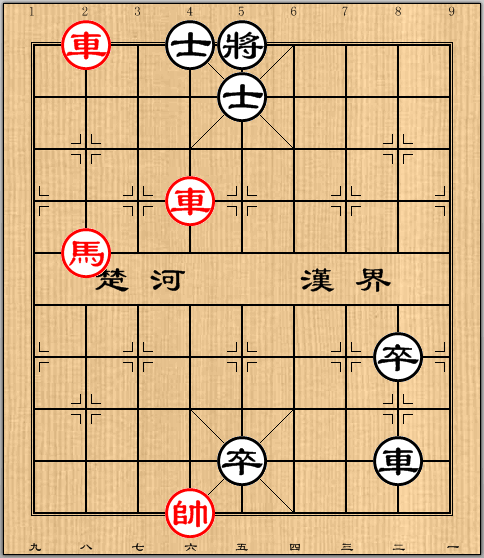
\includegraphics[width=5cm]{pic/钓鱼马-如何构造钓鱼马杀型又一例.png}
\caption{钓鱼马-如何构造钓鱼马杀型又一例}
\end{figure}


这一局中黑将居于原位,双士联结。不过此刻红马瞄准钓鱼马位跃跃
欲试,同时集结双车、帅三子瞄准黑方的底士,可以强行突破,形成
钓鱼马杀法。招法如
下:

\begin{verbatim}
1. 车八平六,士5退4
2. 车六进三,将5进1
3. 马八进七,将5进1 [注1]
4. 车六退二,将5退1
5. 车六退三,将5进1
6. 马七进六,将5退1 [注2]
7. 车六平五。红胜。
      
[注1]:此刻黑方如果将5平6,红方可以马七退五,将6平5,马
五进三,红胜。在这个变化红方施展“绕圈马”连续将军,实现马
的大范围调动。

[注2]: 当红方出帅助攻时,由钓鱼马位转至虎穴马位是一种常
用的手段。参见下图。
\end{verbatim}

\begin{figure}[H]
\centering
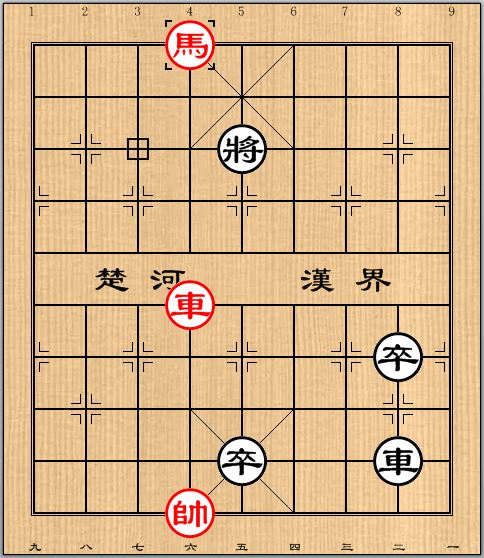
\includegraphics[width=5cm]{pic/钓鱼马转虎穴马借帅力做杀.png}
\caption{钓鱼马转虎穴马借帅力做杀}
\end{figure}


\section{如何消除黑方的选择}
\label{sec-3-3}
\subsection{如何消除黑方的选择例1}
\label{sec-3-3-1}
\begin{figure}[H]
\centering
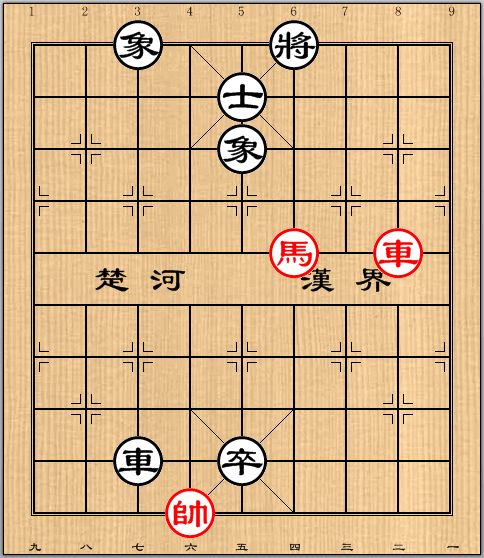
\includegraphics[width=5cm]{pic/钓鱼马-如何消除黑方的选择.png}
\caption{钓鱼马-如何消除黑方的选择例1}
\end{figure}

在\hyperref[sec-3-1]{钓鱼马基础型}中,黑方是有选择的余地的,可以上将也可以进将,只不过无论黑方上将还是进将,红方都可以完
成将杀。但是有的情况下就不是这样了,黑方可以做出有
利于自己的选择。比如下图所示的棋形。
与上面的钓鱼马基础性相比较,主要的区别是黑方多了一个中
士,当红方马四进三将的时候:
\begin{itemize}
\item 黑方如果走将6平5,那么红方正好可以误打误撞走车二进四完成将杀;
\item 但是如果黑方机警地走将6进1,那么红方车二平四将就不是杀了,黑方可以上士挡。
\end{itemize}

可见当红方钓鱼马将军的时候, \textbf{黑方上将通常是比进将更为顽强的
选择} ,因为如果进将的话,黑方就必须防范红车的底线将军,而红
车和红马都瞄准着黑方的底士角位,红方是很容易突破黑方的这道防
线的,而上将就不一样了,即使只有一个孤士,也可以防范住红车的
纵向攻击。不过如果看硬币的另外一面,红方的钓鱼马有逼迫黑方把
将位走高,同时牵制黑方中士的功效。

那么红方是否有破敌良策呢,答案是肯定的。在钓鱼马的
基础型中,我们提到 \textbf{钓鱼马配合高车可以连杀黑方底士角
位的光将} 。但钓鱼马的威力不止于此,当红车处于下二
路或者处于中路时,此时的车虽然只可以在纵向或者横向
一个方向上打将,并不是一个严格意义上的高车,却仍然
可以采用钓鱼马的杀法取胜。因为当红车位于下二路的时候,正好限
制了黑将上将的选择,黑将只能进将,在此情况下,红车只要可以横
向打将就够了;而当红车处于
中路时,正好限制了黑将进将的选择,黑方只能上将,在此情况下红
车只要能纵向打将就够了。

在这里我们也可以体会一下车的用法,我们是要用车直接对黑将发起
攻击,还是要车控制黑将。如果要用车直接发起攻击,通常需要保持
车在高位,而如果要用车控制黑将,通常需要把车走到贴近黑将的位
置,即把车的位置走低。而车得帅助攻之所以威力大增,是因为得帅
助攻时红车既可以直接对黑将发起攻击,又可以控制黑将,还可以根
据需要在“攻击模式”和“控制模式”之间自由切换。

所以对于底士角位的光将,
以下攻击阵型皆可取胜:
\begin{itemize}
\item 钓鱼马+高车,高车可纵横两路打将;
\item 钓鱼马+中路高车,中路高车虽然仅可以纵向打将,但
由于中路高车限制了黑方进将的选择,可以纵向打将就
够了。
\item 钓鱼马+下二路高车,下二路高车虽然仅可以横向打将,
但由于下二路高车限制了黑方上将的选择,可以横向打
将就够了。
\end{itemize}



在钓鱼马的攻击阵型下, \textbf{红方常可以主动出击,消除黑方的选择空
间} 。这一局红方的招法如下:

\begin{verbatim}
1. 车二进四,将6进1
2. 车二退一,将6退1
3. 马四进三,将6平5
4. 车二进一,红胜。
\end{verbatim}

读者可能会问:“第2回合红方车二退一的时候,黑方为什么不将6
进1逃脱红方钓鱼马的马脚?”因为红方可以马四进六或马
四进二杀,由此可见红方第1、2回合打将顿挫之妙。

\subsection{如何消除黑方的选择例2}
\label{sec-3-3-2}
\begin{figure}[H]
\centering
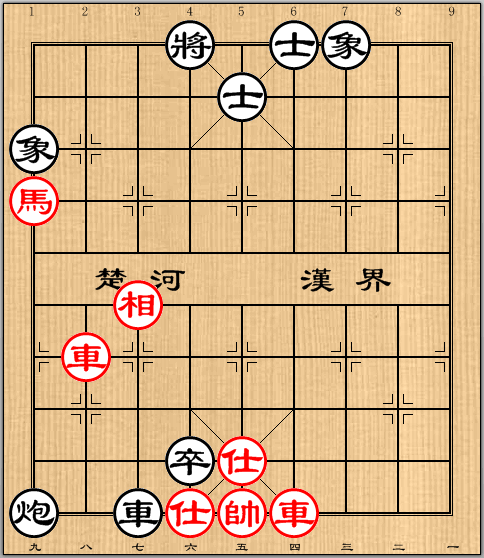
\includegraphics[width=5cm]{pic/钓鱼马-如何消除黑方的选择又一例.png}
\caption{钓鱼马-如何消除黑方的选择例2}
\end{figure}


在\texttt{如何消除黑方的选择例1}的例子中,我们是通过进车打将的顿挫,使得红方的高车先
行控制黑方的下二路,从而消除黑方上将的选择的。但是在上图所
示的选择中,红方无法使用这一手段,因为黑将可以径直升至
三楼,红方无连续进攻的手段。

如果红方直接跳马将呢?
\begin{itemize}
\item 黑方如果将4平5,那么红方当然可以车八进六杀;
\item 但黑方可以上将,红方如果车八平六将,黑方可以士5
进4挡将。如果没有这个中士,红方的车八平六就是杀棋了。
\end{itemize}

可见 \textbf{黑方的中士发挥了关键的防守作用} ,肩负了防范
钓鱼马的重任,不能擅离职守,所以黑方的6路底士其实
是处于无根的状态。

由此思路出发,红方的四路车可以先行 \textbf{车四进九砍底士} ,黑方只能将4
进1,红方可以车八平六将,黑方只能士5进4,红方再车六退一,
黑方将4退1,红方车六进五,将4平5,车六平五,将5平4,马
九进七即可完成绝杀。

从这一局总结的棋理是 \textbf{黑方的中士对钓鱼马是具备防守
力的} ,即黑方的中士是不利于钓鱼马的进攻的。但是如
果看硬币的另外一面, \textbf{红方的钓鱼马也可以对黑方的中
士产生牵制力,让其失去对士角位的看护能力} 。


\subsection{如何消除黑方的选择例3}
\label{sec-3-3-3}
\begin{figure}[H]
\centering
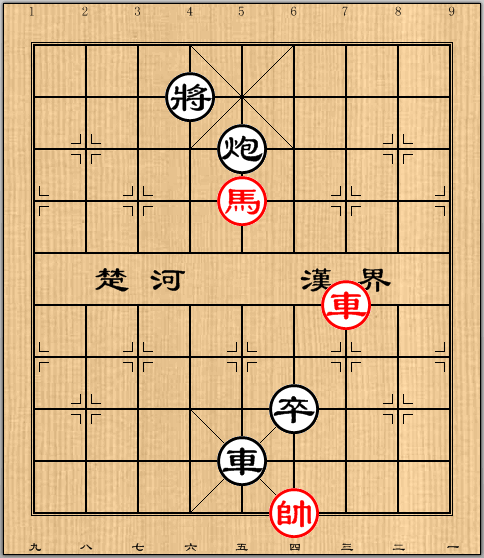
\includegraphics[width=5cm]{pic/钓鱼马-如何消除黑方的选择再一例.png}
\caption{钓鱼马-如何消除黑方的选择例3}
\end{figure}

如图所示为钓鱼马做杀的一个例子,黑方九宫内虽有一炮,却无法发
挥防守作用,反而起了堵塞将路的负作用。如果把黑炮换成马或者象,
那么红方的进攻招法都不成立。可见黑炮不但没有起到防守作用,反
而成了红方的“援军”。

\begin{verbatim}
1. 车三进四,将4退1
2. 马五进七,将4平5
3. 车三进一。红胜。
\end{verbatim}

这一局,红方的招法并不多,贵在次序井然。

\section{如何突破对方的防守}
\label{sec-3-4}
\subsection{钓鱼马-突破黑方对底线的防守}
\label{sec-3-4-1}
\begin{figure}[H]
\centering
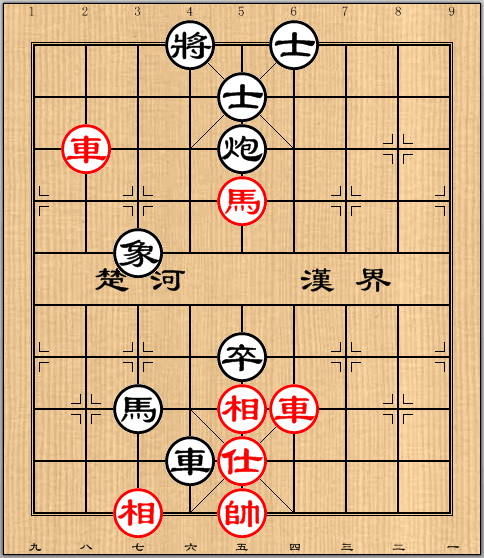
\includegraphics[width=5cm]{pic/钓鱼马-突破黑方对底线的防守.png}
\caption{钓鱼马-突破黑方对底线的防守}
\end{figure}

如图所示的局面中,红方的中马还是可以接着将军的先手跳到
钓鱼马的马位。黑方可以上将,红方无法肋线打将。所以
红方首先需要消除黑方上将的选择。

可以参考前面介绍的打将顿挫的手法控制下二路,
招法是车八
进二打将,黑方将4进1,红方再车八退一打将,黑方无法将4进
1,否则红方可以马五退七杀,黑方只能将4退1,这样红方八路
车控制了下二路,再马五进七钓鱼马将的时候,黑方就只能进
将了。

但是此处红方如果再车八进一,却无法成杀了,因为黑方的4路
肋车和中士合力将空虚的底线守护住了,红方车八进一将的时
候黑方可以士5退4挡将。

尽管如此,红方还是有突破的手段,既然黑方的中士肩负着防
守底线的重任,那么黑方的6路底士其实是处于无根的状态,所
以红方可以直接车四进七砍底士,黑方如果落士吃,那么红方
前面的招法就成立了,可以车八进二,将4进1,车八退一,将4
退1,马五进七,将4平5,车八进一,车4退8,车八平六胜。黑
方如果上将的话,红方可以车八退一,将4进1,马五退七
杀。

可以将这一局和 \ref{sec-3-3-2}一节结合
起来,体会 \textbf{钓鱼马对黑方中士的牵制力} 。

\subsection{钓鱼马-消除对方的防御力量}
\label{sec-3-4-2}
\begin{figure}[H]
\centering
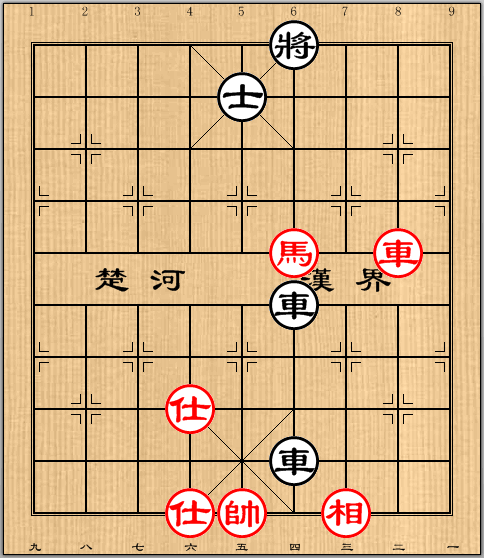
\includegraphics[width=5cm]{pic/钓鱼马-消除对方的防御力量.png}
\caption{钓鱼马-消除对方的防御力量}
\end{figure}


如图所示的局面,黑方在6路肋道上集结了双车,牢牢守护住了
肋道和底线士角位,当红方卧槽马将时,黑方无论是上将还是
下将,红方都无法直接做杀。那么红方如何突破呢?招法如下:

\begin{verbatim}
1. 车二进四,将6进1
2. 车二退一,将6退1 [注1]
3. 马四进三,将6平5
4. 车二平五,将5平4 [注2]
5. 车二进一,将4进1
6. 马三退五,将4进1 [注3]
7. 马五退七,将4退1
8. 马七进八,将4进1
9. 车五平六,红胜。

[注1]:通过打将顿挫控制下二路。

[注2]:带将吃士。

[注3]:车帅限制黑将活动空间后开始施展“绕圈马”。
\end{verbatim}

从以上招法可见,红方可以先利用打将顿挫控制下二路,再用
钓鱼马把黑将逼回原位,然后车带将吃去中士,车借帅力控制
中路之后,把黑将限制在4路肋道上,然后施展“绕圈马”,借
助连续将军的先手,实现了马的大范围转移,最终以白脸将的
杀法取胜。此局红方并无精妙之招,贵在次序井然,使得车马帅三子
取得密切配合。

\textbf{此局中尤其需要体会的是限制黑将活动空间后,绕圈马
连续将军调整位置的手段,这是车马冷招的常见手段。}


\section{钓鱼马和卧槽马之间的联系}
\label{sec-3-5}
\subsection{钓鱼马和卧槽马之间的联系例1}
\label{sec-3-5-1}
\begin{figure}[H]
\centering
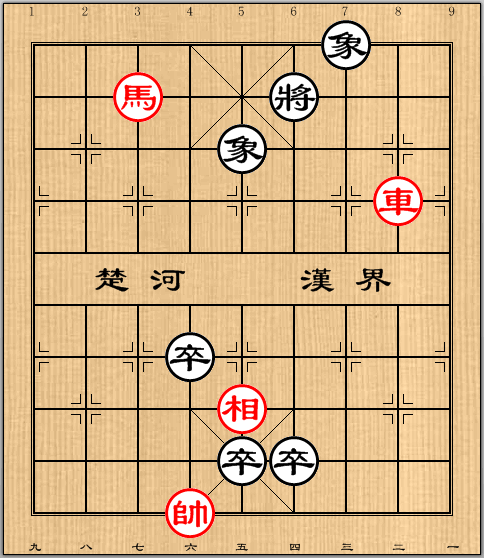
\includegraphics[width=5cm]{pic/卧槽马和钓鱼马之间的联系.png}
\caption{钓鱼马和卧槽马之间的联系例1}
\end{figure}


卧槽马可以通过高位 \textbf{花心马、天马} 等马位调整至钓鱼马马位。这一局招法虽然不多,但是
借此可以体会如何诸多运马技巧:
\begin{itemize}
\item 卧槽马限制将位后如何利用打将顿挫来调整车的位置;
\item 车带着催杀的先手消除对方的防御子力以发挥帅力;
\item 如何大范围调整马的位置。
\end{itemize}

\begin{verbatim}
1. 车二进二,将6退1
2. 车二退五,将6进1
3. 车二平四!,将6平5。[注1]
4. 车四平六,将5平6
5. 马七退六,将6退1
6. 马六退四,将6进1。[注2]
7. 车六进五,将6进1。[注3]
8. 马四进二。红胜。
   
[注1]:先车二平四打将再车四平六吃卒,走得准确。把黑将打
到花心位后,车四平六吃卒也成了先手,下伏车六进五再车六
平四杀。

[注2]:马六退四至河口,该马位我称之为天马位,因其大范围
转移如天马行空。天马的功效和炮位马有诸多相似之处,读者
可以联系起来体会。

[注3]:若将6退1,红方可以马四进三,将6平5,车六进一杀。
\end{verbatim}



\subsection{钓鱼马和卧槽马之间的联系例2}
\label{sec-3-5-2}
\begin{figure}[H]
\centering
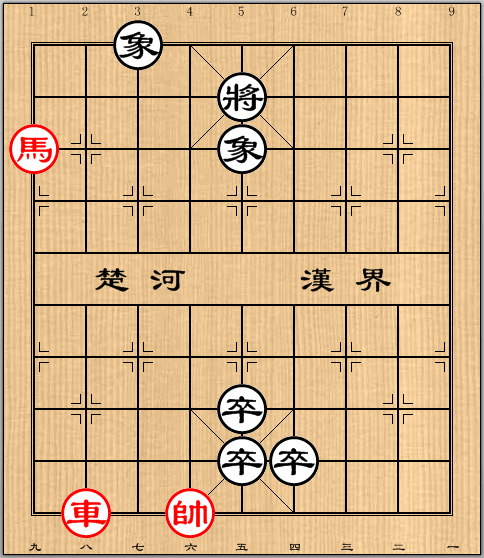
\includegraphics[width=5cm]{pic/卧槽马和钓鱼马之间的联系又一例.png}
\caption{卧槽马和钓鱼马之间的联系例2}
\end{figure}


本局面和\texttt{钓鱼马和卧槽马之间的联系例1}有诸多相似之处,可以采用
类似的方法取胜。招法如下:

\begin{verbatim}
1. 车八进八,将5退1
2. 马九进七,将5平6
3. 车八退五,将6进1
4. 车八平四!,将6平5
5. 车八平六!,将5平6
6. 马七退六,将6退1
7. 马六退四,将6进1
8. 车六进五,将6退1
9. 马四进三,将6平5
10. 车六进一。红胜。
\end{verbatim}

以上这段招法的取胜思路和上一局如出一辙,还是借助卧槽马调整车
位,直至形成车帅一线+卧槽马的阵型。

除了把车调整至六路借帅力外,还可以将车调整至黑方的空虚的右翼,
也可以取胜,招法如下:

\begin{verbatim}
1. 车八进八,将5退1
2. 马九进七,将5平6 [注1]
3. 车八退四,将6进1
4. 车八平四,将6平5
5. 车八平二,将5平6 [注2]
6. 马七退六,将6退1
7. 马六退四,象5退7
8. 马四进三,将6平5
9. 车二平四。   
   
[注1]:如果将5进1,红方可以马七退六,将5退1,马六进四,
将5平6,车八平五,以花心车做杀。

[注2]:连续三步运车,把红车运至黑方防守薄弱的一翼。
\end{verbatim}

\subsection{钓鱼马和卧槽马之间的联系例3}
\label{sec-3-5-3}
在\ref{sec-3-5-1}节中,第7回合,红方车六进五,黑
方上将,红方的马四进二之所以能完成绝杀,主要原因是黑方的中象
限制了将路,在此试问,如果黑方没有中象的话,红方是否可以取胜
呢。我们从第4回合之后的棋形出发(移除了黑方的中象),如下图
所示。

\begin{figure}[H]
\centering
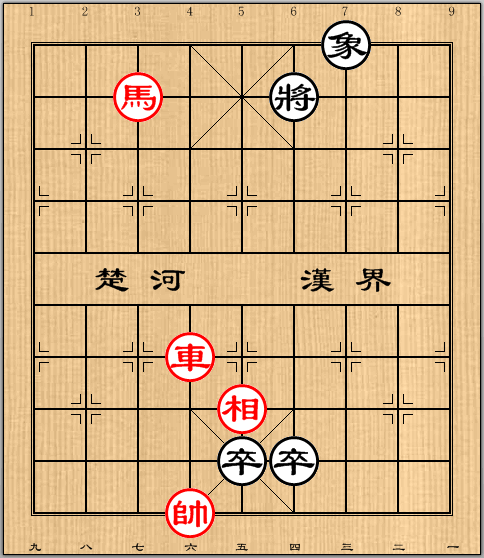
\includegraphics[width=5cm]{pic/卧槽马和钓鱼马之间的联系-车位调整.png}
\caption{卧槽马和钓鱼马之间的联系例3}
\end{figure}

此处,如果黑方没有7路底象,红方可以采用\texttt{钓鱼马和卧槽马之间的
联系例2}中的第2种招法取胜,即

\begin{verbatim}
1. 车六平四,将6平5
2. 车四平二,将5平6
3. 马七退六,将6退1
4. 马六进四,将6进1
5. 车二进五,将6进1 [注1]
6. 马四进六,将6平5 
7. 车二退一。

[注1]:黑方没有7路底象,如果将6进1的话,红方可以马四进三,
将6平5,车二进一杀。
\end{verbatim}

但即使黑方有7路底象防守左翼的底线,红方可以把车调动到黑方的
右翼,再以\texttt{钓鱼马和卧槽马之间的联系例2}中的第2种方法取胜。
红方的招法如下:

\begin{verbatim}
1. 马七退六,将4退1
2. 车六平四,将4平5
3. 车四平八,将5平6。[注1]
4. 马六退四,将6进1
5. 车八进五,将6退1
6. 马四进三,将6平5
7. 车八进一。红胜。

[注1]:借助花心马调整车位。如果将5平4,红方可以车八平六,下
伏马六进七,将5进1,车六进五,将5退1,车六平四杀,黑方必须应
对,有以下几种选择:
- 将4平5,红方还是可马六进七,将5进1,车六进五,将5退1,车六
  平四杀。
- 将4进1,红方也还是可以马六进七,将4平5,车六进五,将5退1,
  车六平四杀。
\end{verbatim}

可见红车除了可以借助卧槽马来调整位置,还可以借助花心马来调整
位置,并且还可以调整到借助卧槽马无法抵达的位置。此局中,红马
如果再卧槽马位,红方车四平八这步棋并不是先手,但当红马在花心
马时,红方车四平八这步棋就是先手了。此处需细心体会花心马的妙
用。

\subsection{钓鱼马和卧槽马之间的联系例4}
\label{sec-3-5-4}
如果对\ref{sec-3-5-3}的棋形略作修改,增加
一个3路底象,那么红方是否可以取胜呢?

\begin{figure}[H]
\centering
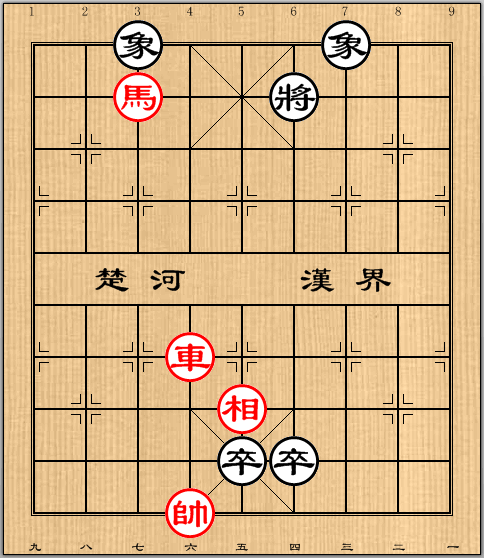
\includegraphics[width=5cm]{pic/卧槽马和钓鱼马之间的联系-车位调整又一例.png}
\caption{卧槽马和钓鱼马之间的联系-车位调整又一例}
\end{figure}

答案是肯定的。红方取胜的招法如下:
\begin{verbatim}
1. 马七退六,将6退1
2. 车六平四,将6平5
3. 车四平三,将5平6 [注1]
4. 车三进六,将6进1 [注2]
5. 车三退六,将6退1
6. 车三平四,将6平5
7. 车三平二,将5平6 [注3]
8. 马六退四,将6进1
9. 车二进五,将6进1
10. 马四进六,将6平5
11. 车二退一。红胜。

[注1]:形成了卧槽马配合高车的阵型,黑将必须调整位置。

[注2]:红方先手吃去底象,破除了黑方的底线的防守力量。

[注3]:通过第6回合和第7回合的顿挫,红方把车调整到二路,有利
于与钓鱼马的配合,避免将来钓鱼马挡住红车进底线打将的线路。
\end{verbatim}

此外,红方还有一路比较简洁的取胜方法,以花心车杀法取胜。

\begin{verbatim}
1. 马七退六,将6退1
2. 马六退四,将6进1
3. 车六进五,将6进1
4. 车六平五,卒6进1
5. 马四进六。红胜。
\end{verbatim}


\section{钓鱼马和拔簧马的结合}
\label{sec-3-6}
\subsection{钓鱼马和拔簧马的结合例1:借帅力转虎穴马做杀}
\label{sec-3-6-1}
\begin{figure}[H]
\centering
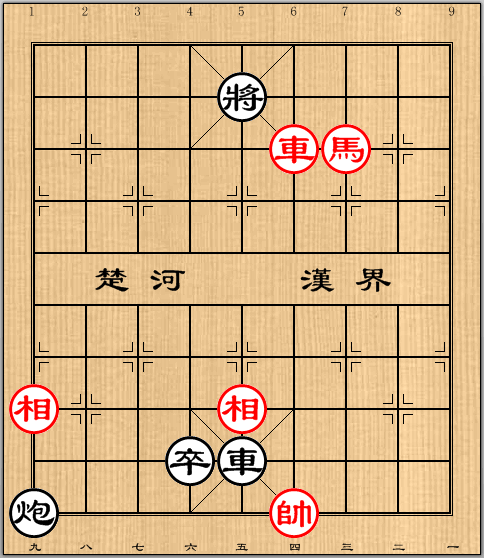
\includegraphics[width=5cm]{pic/钓鱼马-借帅力转虎穴马做杀.png}
\caption{钓鱼马-借帅力转虎穴马做杀}
\end{figure}

如图所示的棋形红车可以借助拔簧马的抽闪调整位置。红方有两种取
胜的招法,一种横向调整车位,一种是纵向调整车位。

纵向调整车位的进攻招法如下:
\begin{verbatim}
1. 车四退三,将5进1
2. 马三进四,将5退1
3. 车四平五。
\end{verbatim}

横向调整车位的进攻招法如下:
\begin{verbatim}
1. 车四平八,将5平4
2. 马三进四,将4平5
3. 车八平五。
\end{verbatim}

下面再来看一个“借帅力转虎穴马”做杀的例子,见图\ref{dym-jslzhxmzs-yyl}。

\begin{figure}[H]
\centering
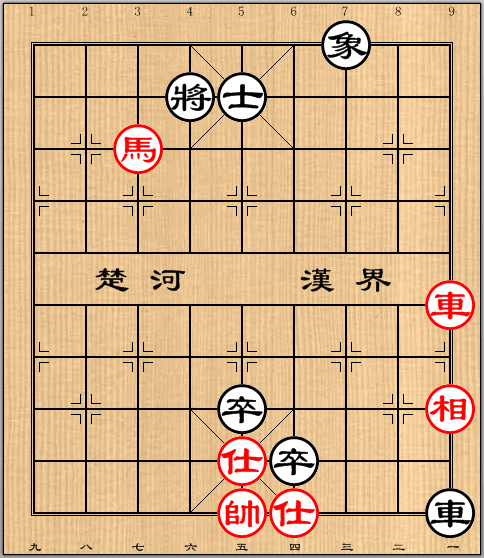
\includegraphics[width=5cm]{pic/钓鱼马-借帅力转虎穴马做杀-又一例.png}
\caption{\label{dym-jslzhxmzs-yyl}钓鱼马-借帅力转虎穴马做杀-又一例}
\end{figure}

招法如下:

\begin{verbatim}
1. 车一平六,士5进4
2. 帅五平六,卒5进1
3. 车六进三,将4平5
4. 车六退三,将5进1
5. 马七进六,将5退1
6. 车六平五,象7进5
7. 车五进三。红胜。
\end{verbatim}

\subsection{钓鱼马和拔簧马的结合例2}
\label{sec-3-6-2}
\begin{figure}[H]
\centering
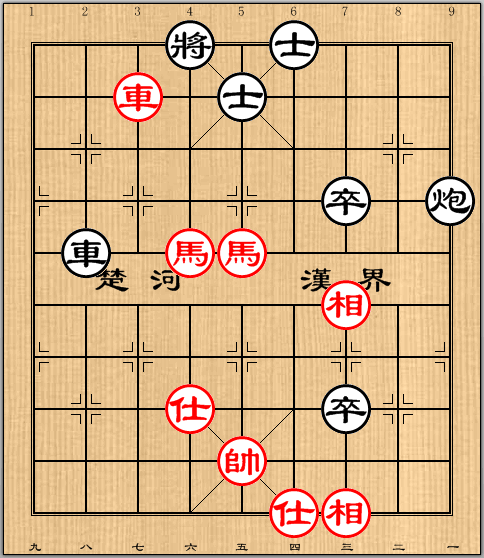
\includegraphics[width=5cm]{pic/钓鱼马和拔簧马的结合例2.png}
\caption{钓鱼马和拔簧马的结合例2}
\end{figure}

如图所示的棋形也是钓鱼马和拔簧马结合的例子。红方的
招法如下:
\begin{verbatim}
1. 马五进四,士5进6
2. 马六进七,车2平5
3. 相三进五,车5平3
4. 车七进一,将4进1
5. 车七平六。红胜。
\end{verbatim}

\section{钓鱼马-弃车改变黑方的将门位置}
\label{sec-3-7}
\begin{figure}[H]
\centering
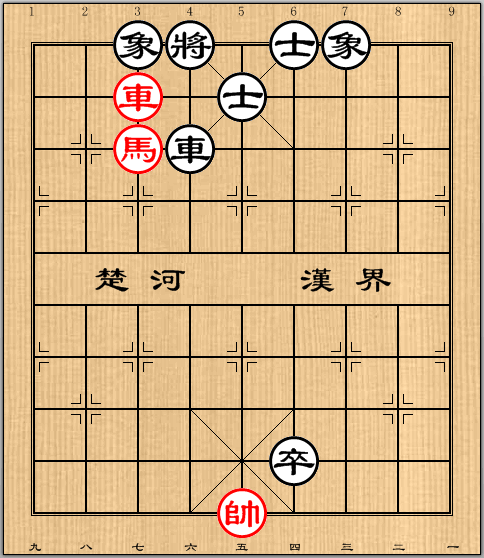
\includegraphics[width=5cm]{pic/钓鱼马-弃车改变黑方的将门位置.png}
\caption{钓鱼马-弃车改变黑方的将门位置}
\end{figure}

在卧槽马一章我们介绍过弃车改变黑方将门的位置再做杀的手
段,在钓鱼马中也存在类似的手段,如下图所示的棋形。

\begin{verbatim}
1. 车七进一,将4进1
2. 车七平六,士5退4
3. 马七进八。红胜。
\end{verbatim}



\chapter{高钓马}
\label{sec-4}
位于黑方3卒位或者7卒位的马被称为高钓马,这个位置的马比
钓鱼马高了一格,所以叫高钓马。高钓马同时控制了九宫的两
条边的中点,当黑将在外,且补有中士导致无法进将时,高钓
马阵形有很强的进攻力。

\section{侧面虎的基础型}
\label{sec-4-1}
\begin{figure}[H]
\centering
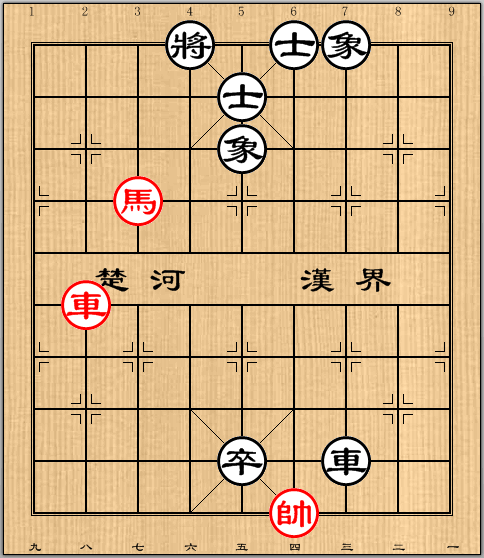
\includegraphics[width=5cm]{pic/侧面虎的基础型.png}
\caption{\label{cmhjcx1}侧面虎的基础型-1}
\end{figure}

如图\ref{cmhjcx1}所示为侧面虎的基础型-1,红方可以车八进五,象5退3,车
八平七成杀。

图\texttt{侧面虎的基础型-2}所示的是侧面虎的另一个常见的棋形,红方有两路招法都
可以取胜:
\begin{itemize}
\item 一路是车七平八,将4退1,车八进二。
\item 另一路是车七进一,将4进1,车七平六。
\end{itemize}


\begin{figure}[H]
\centering
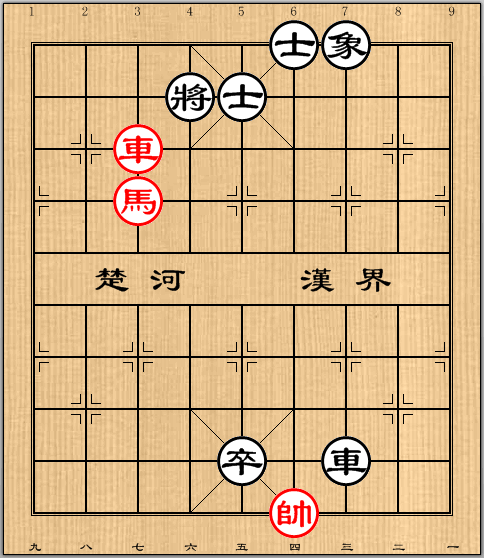
\includegraphics[width=5cm]{pic/侧面虎的基础型-2.png}
\caption{侧面虎的基础型-2}
\end{figure}


实战中有的时候并不是两路招法都是可行的,需要依据局面进
行选择。

\section{侧面虎-如何构造侧面虎杀型}
\label{sec-4-2}
\subsection{弃兵成侧面虎}
\label{sec-4-2-1}
如图所示,为胡荣华和杨官璘的实战,胡荣华执红,杨官
璘执黑。黑将在外,红马处于中象位,可以立刻转战至高
调马位,红方显然存在高钓马的杀型。但是红兵妨碍的红
马威力的发挥,红方可以先手弃兵后以钓鱼马杀法取胜。

\begin{figure}[H]
\centering
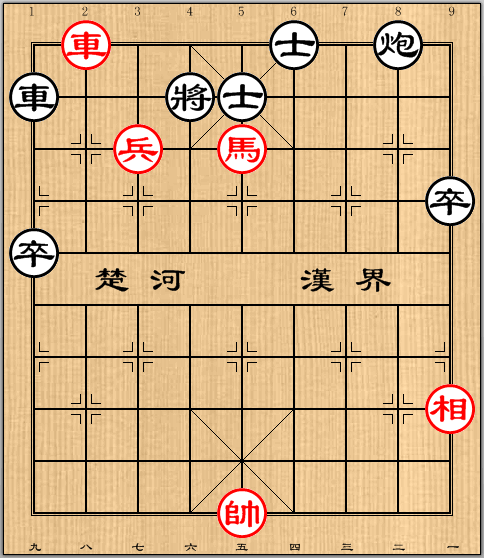
\includegraphics[width=5cm]{pic/弃兵成侧面虎.png}
\caption{弃兵成侧面虎}
\end{figure}


\begin{verbatim}
1. 兵七平六,将4进1
2. 车八退二,将4退1
3. 马五退七,将4退1
4. 车八进二。红胜。
\end{verbatim}

\subsection{如何防止黑方进将}
\label{sec-4-2-2}
\begin{figure}[H]
\centering
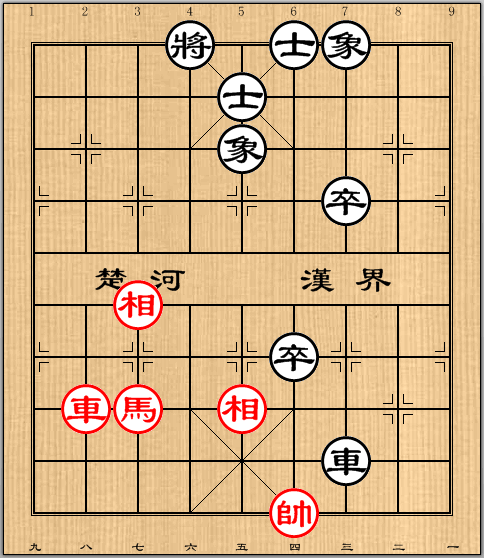
\includegraphics[width=5cm]{pic/侧面虎-如何放置黑方进将.png}
\caption{侧面虎-如何放置黑方进将}
\end{figure}

红方侧面虎的杀势能够成立的一个
重要前提是黑方自己补起了中士,阻断了黑将进将逃跑的通道,
因此面对红方侧面虎的杀势,黑方一定会试图移开中士解杀,
红方该如何阻止黑方的这一计划呢,可以看看下图所示的例子。
红方的招法如下:

\begin{verbatim}
1. 车八进七,将4进1
2. 马七进六,士5进6
3. 车八平五,士6退5
4. 马六进七,将4进1
5. 车五平八。红胜。
\end{verbatim}

\section{如何突破黑方的防守}
\label{sec-4-3}
\subsection{侧面虎-如何破除中象对底线的防御}
\label{sec-4-3-1}
\begin{figure}[H]
\centering
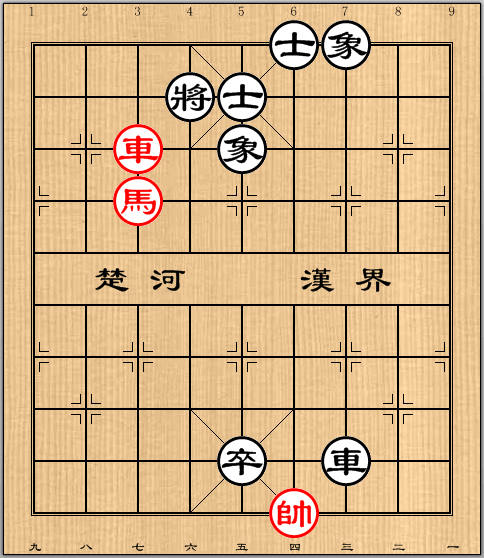
\includegraphics[width=5cm]{pic/侧面虎-如何破除中象对底线的防御.png}
\caption{侧面虎-如何破除中象对底线的防御}
\end{figure}

如图所示局面,黑方的中象防守住了3路底象位,红方如果贸然
车七进一,黑方将4退1,黑方就转危为安了。红方正确的招法
是:

\begin{verbatim}
1. 车七平八,将4退1
2. 车八进二,象5退3
3. 车八平七。红胜。
\end{verbatim}

\subsection{侧面虎-如何避免黑炮的防御}
\label{sec-4-3-2}

\begin{figure}[H]
\centering
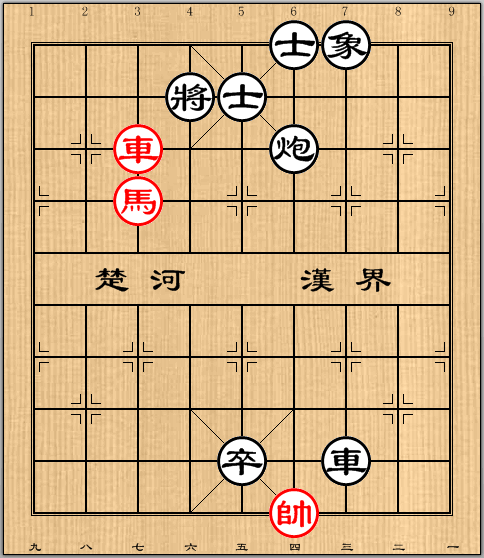
\includegraphics[width=5cm]{pic/侧面虎-如何破除黑炮的防御.png}
\caption{侧面虎-如何避免黑炮的防御}
\end{figure}


如图所示局面,黑方布置线的炮可以垫马脚,红方如果车七平
八,黑方可以炮6平3蹩马脚,红方固然可以车八平七吃炮,但
是黑方以牺牲黑炮为代价延缓了红方的进攻速度,争取了进攻
的时间,可以抢先动手成杀,在红方车八平七吃炮后黑方接走车7进1
或者车7平6即可取胜。

红方正确的招法是:

\begin{verbatim}
1. 车七进一,将4进1
2. 车七平六。红胜。
\end{verbatim}

\subsection{侧面虎-如何消除黑方的防御子力}
\label{sec-4-3-3}
\begin{figure}[H]
\centering
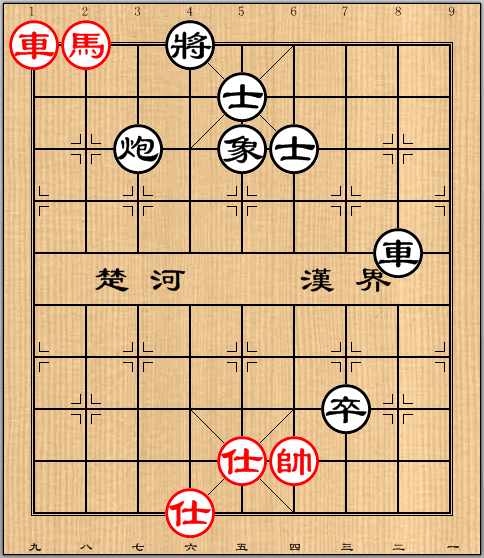
\includegraphics[width=5cm]{pic/侧面虎-如何消除黑方的防御子力.png}
\caption{侧面虎-如何消除黑方的防御子力}
\end{figure}


如图所示局面中,如果没有黑炮,那么红方可以简单取胜,招
法是马八退九,将4进1,马九退七,将4进1,车九退二。

但是由于黑炮在布置线,导致红方马九退七不是将军了。那么
红方是否可以连杀呢?答案是肯定的,招法如下,大家可以借
助此局体会如何借车使马。

\begin{verbatim}
1. 马八退七,将4进1
2. 马七进八,将4退1
3. 马八退九,将4进1
4. 马九退七,将4进1
5. 车九退二。红胜。
\end{verbatim}

本局中红车以及黑方的中士限制了黑将的活动空间,为红方实战“绕
圈马”变位创造了条件。

\subsection{侧面虎-如何破除黑车对底线的防御}
\label{sec-4-3-4}
\begin{figure}[H]
\centering
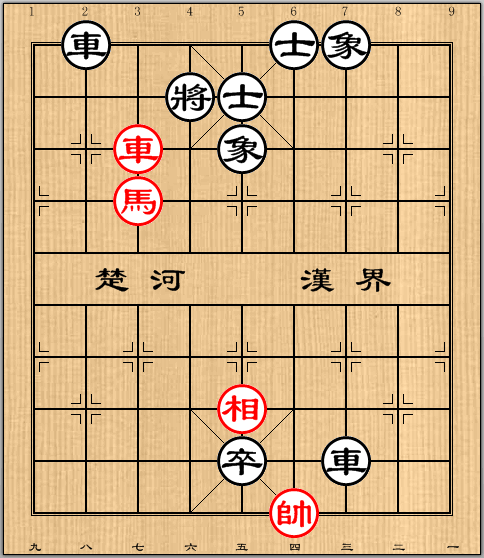
\includegraphics[width=5cm]{pic/侧面虎-如何破除黑车对底线的防御.png}
\caption{侧面虎-如何破除黑车对底线的防御}
\end{figure}


将如图所示的局面和侧面虎的基础型进行比较,可以发现主要
的区别是黑方在底线布置了车进行防御。但红方可以巧妙地突破
这道防线,关键是借拔簧马抽闪之际把红车和黑车对上,招法如下:

\begin{verbatim}
1. 车七平八,将4退1
2. 车八进二,象5退3
3. 车八平七。红胜。
\end{verbatim}

\section{高钓马-闷杀}
\label{sec-4-4}
\begin{figure}[H]
\centering
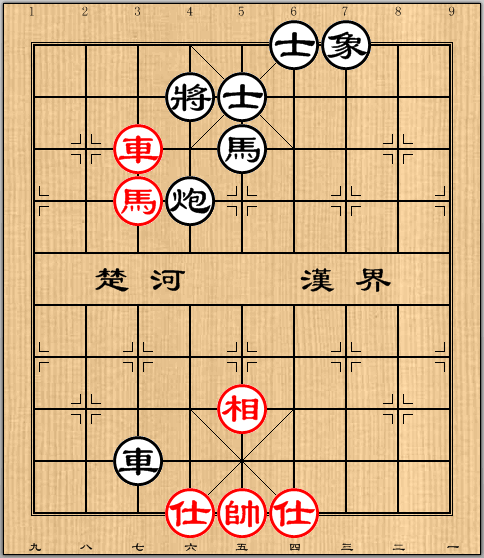
\includegraphics[width=5cm]{pic/高钓马-闷杀.png}
\caption{高钓马-闷杀}
\end{figure}

与在卧槽马和钓鱼马一章介绍的一些棋例类似,高钓马也可以通过弃
车来做闷杀。

\begin{verbatim}
1. 车七进一,将4进1
2. 车七平六,炮4退2
3. 马七退五。红胜。
\end{verbatim}

\section{高钓马与其他马位的结合}
\label{sec-4-5}
\subsection{挂角马-侧锋马-高钓马}
\label{sec-4-5-1}
如图所示的局面,看似挂角马的杀型,其实是一个高钓马侧面
虎做杀的局面。

\begin{figure}[H]
\centering
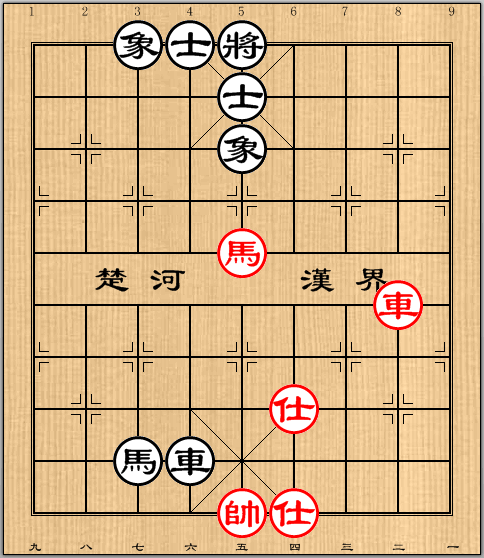
\includegraphics[width=5cm]{pic/侧面虎-挂角马-侧锋马-高钓马.png}
\caption{侧面虎-挂角马-侧锋马-高钓马}
\end{figure}


\begin{verbatim}
1. 车二进五,象5退7。[注1]
2. 马五进四,将5平6
3. 马四进二,将6进1
4. 马二退三,将6退1
5. 车二退二。红胜。   
   
[注1]:如果士5退4,红方马五进四,将5进1,车二退一,可以
速胜。
\end{verbatim}

从以上的招法可见,红马本来马五进三,一步就可以跳至高钓
马的位置上,但是为了加快进攻速度,却是通过马五进四、马
四进二、马二退三花了三步棋到达高钓马的位置,在此可以体
会一下运马的技巧,对马而言有时候走直线并不是最快的线路。

\subsection{花心马-挂角马-前锋马-高钓马}
\label{sec-4-5-2}

\begin{figure}[H]
\centering
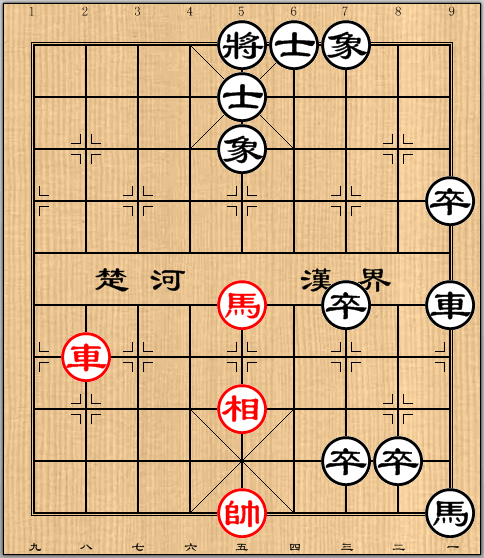
\includegraphics[width=5cm]{pic/花心马-挂角马-前锋马-高钓马.png}
\caption{花心马-挂角马-前锋马-高钓马}
\end{figure}

\begin{verbatim}
1. 马五进六,士5进4 [注1]
2. 马六进四,将5平4
3. 车八进四,将4进1
4. 帅五平六,士6进5 [注2]
5. 马四退五,士5进6
6. 车八进一,将4退1
7. 车八进一,将4进1
8. 车八平五。红胜。
   
[注1]:伏有卧槽马杀,黑方只有士5进4可暂结燃眉之急,如:
- 士5进4,红方可以马六进四挂角杀。
- 将5平4,红方可以车八进六,将4进1,马六进八,将4进1,车八退
  一,象5进7,象五进三。红胜。
  
[注2]:无论是第3回合的车八进四,还是第4回合的帅五平六,都是
为了逼迫黑方补中士,从而便于红方的高钓马进攻。
\end{verbatim}

可以结合图\ref{fxlsgdcl}所示的棋形再体会下本节中的关键招法:
\begin{itemize}
\item 挂角马转前锋马再转高钓马
\item 进车捉高士逼迫黑方上中士
\end{itemize}

\begin{figure}[H]
\centering
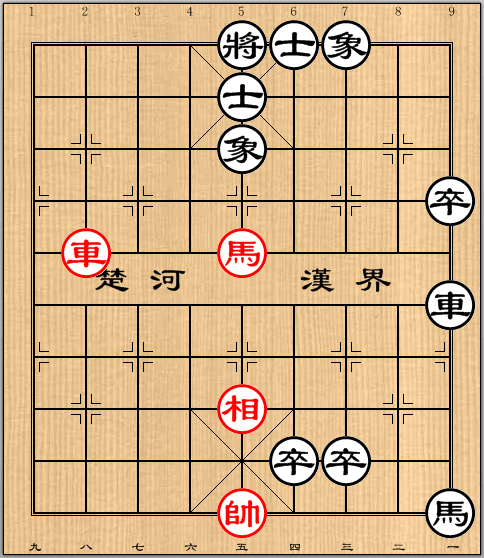
\includegraphics[width=5cm]{pic/飞相露帅隔断车路.png}
\caption{\label{fxlsgdcl}飞相露帅隔断车路}
\end{figure}

图\ref{fxlsgdcl}棋形的招法如下:

\begin{verbatim}
1. 相五进三,士5进4 [注1]
2. 马五进四,将5平4
3. 车八进二,士6进5
4. 车八进二,将4进1
5. 马四退五,士5进6
6. 车八平五,士4退5
7. 马五进七,将4进1
8. 车五平八。红胜。   
   
[注1]:飞相露帅同时隔断车路,发挥中帅的威力的同时限制了黑车
的威力,取胜的关键招法。黑方士5进4是最为顽强的应招,如改走:
- 置之不理的话,红方可以车八进四将,黑方只能象5退3,红方再马
  五进四,将5平4,马四进二,将4进1,马四退三高钓马杀;
- 士5进6或士5退4,红方可以马五进四杀;
- 将5平4,红方可以车八进四,将4进1,马五进七高钓马杀。
\end{verbatim}

\subsection{花心马辗转至高钓马}
\label{sec-4-5-3}
\begin{figure}[H]
\centering
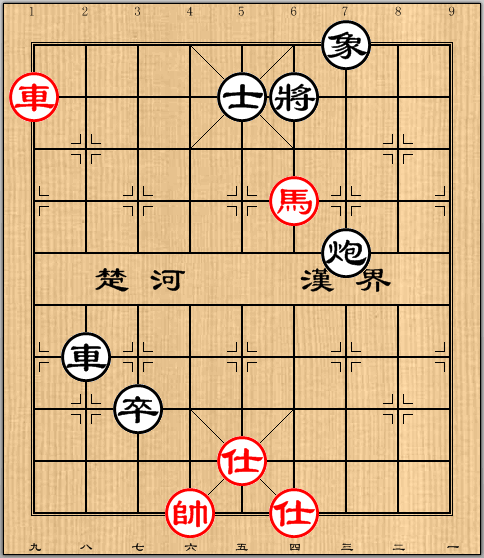
\includegraphics[width=5cm]{pic/花心马辗转至高钓马.png}
\caption{花心马辗转至高钓马}
\end{figure}

此局面并不是一个典型的侧面虎的杀型,首先车是在背面,其次马是
在花心马位,最快也要跳三步才能跳到高钓马位。但是这个棋形中,
花心马辗转至高钓马的过程中,正好三步步步带将,从而可以做成侧
面虎的杀型。

\begin{verbatim}
1. 马四进六,将6进1
2. 马六退五,将6平5
3. 马五进三,将5平6
4. 车九退一。红胜。
\end{verbatim}

\subsection{钓鱼马调整至高钓马}
\label{sec-4-5-4}
\begin{figure}[H]
\centering
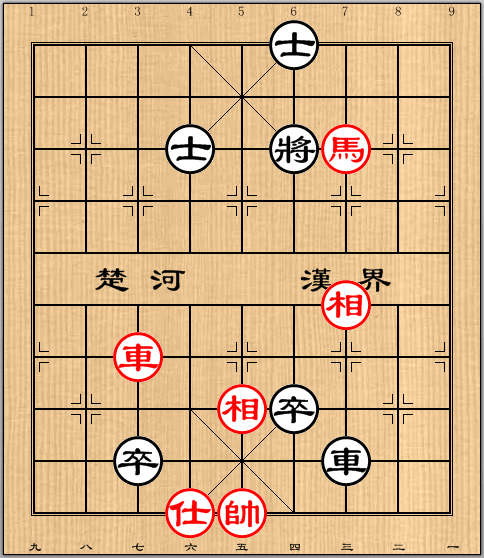
\includegraphics[width=5cm]{pic/钓鱼马调整至高钓马.png}
\caption{钓鱼马调整至高钓马}
\end{figure}

这个局面下,黑方将处于高位,车处于低位,黑6路卒自行阻断了黑
车护肋道的线路,红方明显存在白脸将的杀棋。但红方如果直接相五
退三,黑方可以车7进1抢先做杀。

红方的对策是先行马三退一,伏有车七平四,将6平5,车四平五,将
5平6,马一进二,将6退1,马二退三,将6进1,车五进四高钓马杀的
杀棋。

至此红方存在白脸将和高钓马两路杀棋,黑方不得兼顾。


\begin{verbatim}
1. 马三退一,车7平8。[注1]
2. 相五退三,卒6平5。[注2]
3. 车七平四,将6平5
4. 车四平五,将5平6
5. 车五退一,车8平6
6. 马一进二,将6退1
7. 马二退三,将6进1
8. 车五进四。红胜。

[注1]:下伏车七平四,将6平5,车四平五,将5平6,马一进二,将6
退1,马二退三,将6进1,车五进四的杀棋。黑方只能通过车7平8来
防守,士4退5或者士6进5都是不行的:
- 如果士4退5,红方可以直接马一进二,将6平5,马二进三,将5平4,
  车七平六杀。
- 如果士6进5,红方可以车七平四,将6平5,再马一进二,下伏车四
  平五杀,无解。
  
[注2]:引离黑车后,落相露帅的同时护住底线,正合时宜。黑方弃
卒无奈,目的让出黑车护肋的线路。
\end{verbatim}

\subsection{高钓马-侧锋马转高钓马}
\label{sec-4-5-5}
\begin{figure}[H]
\centering
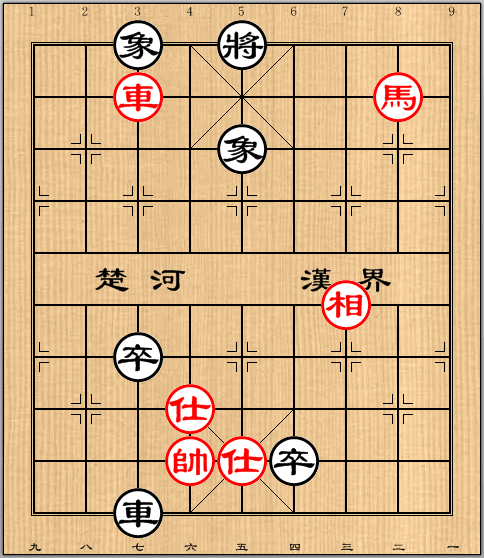
\includegraphics[width=5cm]{pic/高钓马-侧锋马转高钓马.png}
\caption{高钓马-侧锋马转高钓马}
\end{figure}

如图所示的局面,红马可以由二路侧锋马位转移至七路高钓马位做杀,
且看红方是如何实现这一大范围转移的。

\begin{verbatim}
1. 马二退四,将5平4
2. 车七退一,将4进1
3. 车七平五,卒3进1
4. 车五进二,将4进1
5. 马四退五,将4退1
6. 马五进七,将4进1
7. 车五平六。红胜。
\end{verbatim}


\chapter{花心马}
\label{sec-5}
所谓花心马,指的是控制了九宫花心的马,就具体位置而言,
有三个位置,一个是 \textbf{钓鱼马} ,一个是 \textbf{高位花心马} ,一个是 \textbf{低位
花心马} :
\begin{itemize}
\item \textbf{高位花心马} 的马位处于中卒和3卒之间或者中卒和7卒之间。
\item \textbf{低位花心马} 处于黑方的底象位。
\item \textbf{钓鱼马} ,其实是一种特殊的花心马。
\end{itemize}


钓鱼马前面已经单独介绍过了,本章节中我们着重
看高位花心马和低位花心马。

跟 \textbf{花心马} 存在密切关系的两个马位是 \textbf{炮位马} 和 \textbf{天马} ,所
谓炮位马是处于黑方炮位的马,而天马是处于对方沿河线和肋道交叉
点的马:
\begin{itemize}
\item \textbf{炮位马} 既可以奔赴低位花心马马位,又可以奔赴高位花心马马
位;
\item \textbf{天马} 和炮位马类似,同时窥视着 \textbf{高位花心马位} 和 \textbf{钓鱼马
位} 。
\end{itemize}
\section{炮位马}
\label{sec-5-1}
\subsection{炮位马基础型}
\label{sec-5-1-1}

当黑将处于三楼时,红方炮位马配合高车可以产生有效的攻击。

当黑将处于4路士角位时,参见图\ref{pwm-hjz4lsj},红方可以马八进七将:
\begin{itemize}
\item 黑方将4退1则车七平六杀;
\item 黑方将4平5则车七进三杀。
\end{itemize}

\begin{figure}[H]
\centering
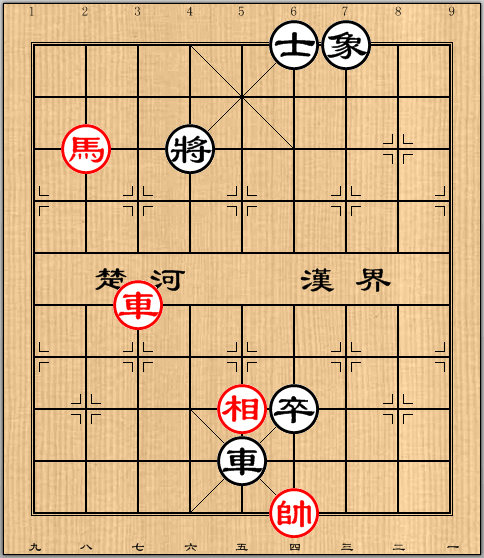
\includegraphics[width=5cm]{pic/炮位马-黑将在4路士角.png}
\caption{\label{pwm-hjz4lsj}炮位马-黑将在4路士角}
\end{figure}

当黑将处于6路士角时,参见图\ref{pwm-hjz6lsj},红方可以马八退六将:
\begin{itemize}
\item 黑方将6退1则车七平四杀;
\item 黑方将6平五则车七进三杀。
\end{itemize}

\begin{figure}[H]
\centering
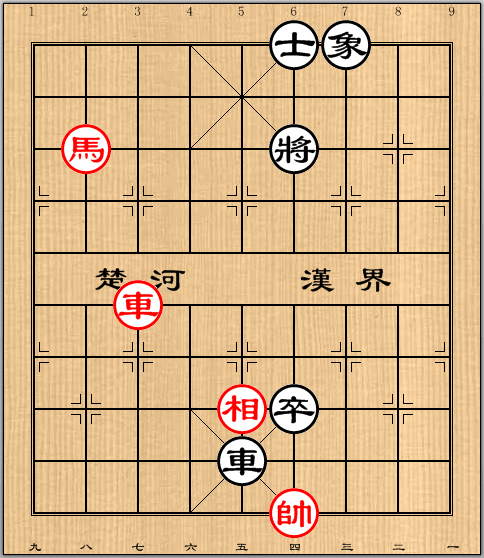
\includegraphics[width=5cm]{pic/炮位马-黑将在6路士角.png}
\caption{\label{pwm-hjz6lsj}炮位马-黑将在6路士角}
\end{figure}

此外红方高车也可以采取钓鱼马一章介绍的打将顿挫的手段来
消除黑方的选择,参见图\ref{pwm-hjz6lsj-yzs}所示的局面。

\begin{figure}[H]
\centering
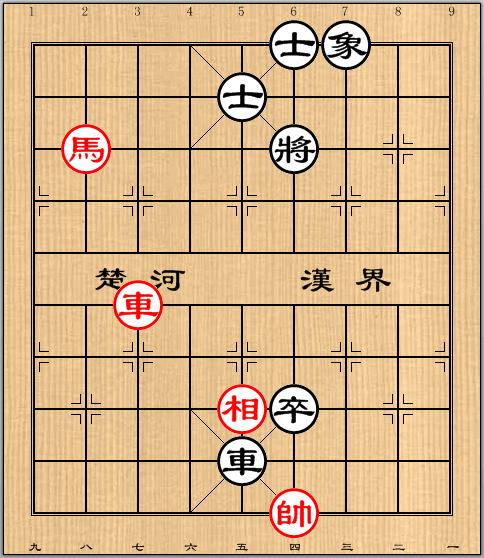
\includegraphics[width=5cm]{pic/炮位马-黑将在6路士角-有中士.png}
\caption{\label{pwm-hjz6lsj-yzs}炮位马-黑将在6路士角-有中士}
\end{figure}


当黑将在6路士角位,并且有中士的时候,红
方如果直接马八退六将,黑方将6平5,红方车八进三将,黑方
可以士5进4挡将,不过红方可以车七平四将,黑方将6平5,再
车四平五将,黑方如果将5平4,红方可以马八进七杀,红方如
果将5平6,黑方可以马八退六杀。红方炮位马的这一灵活性和
后面介绍的天马位的马是类似的,
炮位马同时窥视着低位花心马和高位花心马,而天马是同时窥
视着钓鱼马和高位花心马。

当黑将在中路士,参见图\ref{pwm-hjzzl},红方可以采用中路打将的方式
来逼迫黑方作出选择。无论黑方是将5平4还是将5平6,
红方的炮位马都可以转至低位花心马马位或者高位花心马马位
取胜。

\begin{figure}[H]
\centering
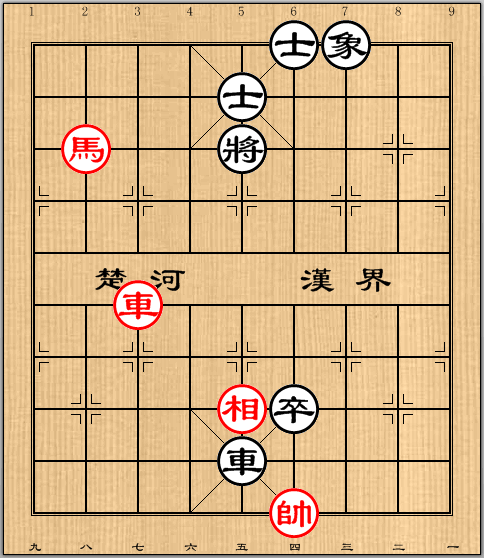
\includegraphics[width=5cm]{pic/炮位马-黑将在中路.png}
\caption{\label{pwm-hjzzl}炮位马-黑将在中路}
\end{figure}


\subsection{炮位马转低位花心马}
\label{sec-5-1-2}
\begin{figure}[H]
\centering
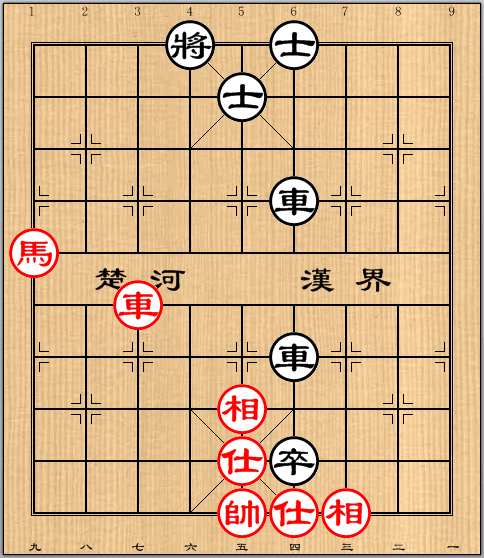
\includegraphics[width=5cm]{pic/炮位马转低位花心马.png}
\caption{炮位马转低位花心马}
\end{figure}

该局面是炮位马转低位花心马的棋例,从该棋例可以看出,炮位马兼
具高钓马和钓鱼马的功效。

\begin{verbatim}
1. 车七进五,将4进1
2. 马九进八,将4进1
3. 车七退二,将4退1
4. 车七退三,将4进1 [注1]
5. 马八进七。红胜。

[注1]:借助拔簧马,把车位走高,形成高车和低位花心马相配合的
阵型,这和高车和钓鱼马相配合的阵型是类似的。
\end{verbatim}

可以再看一个炮位马转低位花心马的例子,参见下图\ref{pwmzdwhxmyyl}。

\begin{figure}[H]
\centering
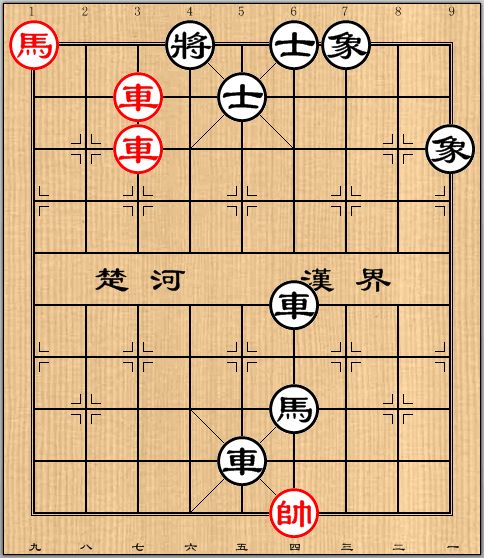
\includegraphics[width=5cm]{pic/炮位马转低位花心马又一例.png}
\caption{\label{pwmzdwhxmyyl}炮位马转低位花心马又一例}
\end{figure}

\begin{verbatim}
1. 前车进一,将4进1
2. 后车进一,将4进1
3. 后车平六,将4退1
4. 马九退八,将4进1
5. 车七退二,将4退1
6. 车七退二,将4进1
7. 马八进七,将4平5,
8. 车七进二,士5进4
9. 车七平六。
\end{verbatim}

\section{天马行空杀法}
\label{sec-5-2}

\subsection{天马星空基础型}
\label{sec-5-2-1}
\begin{figure}[H]
\centering
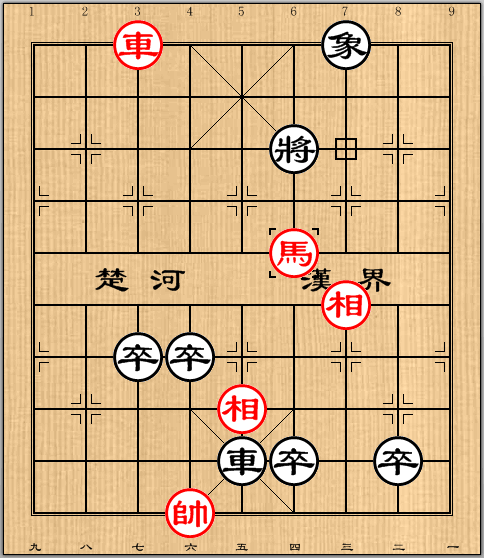
\includegraphics[width=5cm]{pic/天马行空基础型.png}
\caption{天马行空基础型(黑先)}
\end{figure}

如图所示的局面是 \textbf{天马星空} 杀法的基础型。伏有车七平四底线兜
杀的棋,黑方只有将6退1。红方再车七退一:
\begin{itemize}
\item 黑方若将6退1,红方可以马四进三,将6平5,车七进一杀。
\item 黑方若将6进1,红方可以马四进六,将6平5,车七退一杀。
\end{itemize}


之所以称之为 \textbf{天马行空} ,是因为红方的四路马飘在黑将的头顶,
而且河沿地带本来就是整个棋盘的战略高地,称之为 \textbf{天马行空} 恰
如其分。

值得一提的是,红方的车如果不在底线,而处于高位,同样可以构成
天马行空杀法,因为红方伏有马四进六高位花心马将军再高车打将杀
的手段,所以黑方还是必须下将,这样红方又可以车进下二路打将逼
迫黑方表态,再以钓鱼马或者高位花心马做杀。


\subsection{天马行空例1}
\label{sec-5-2-2}
\begin{figure}[H]
\centering
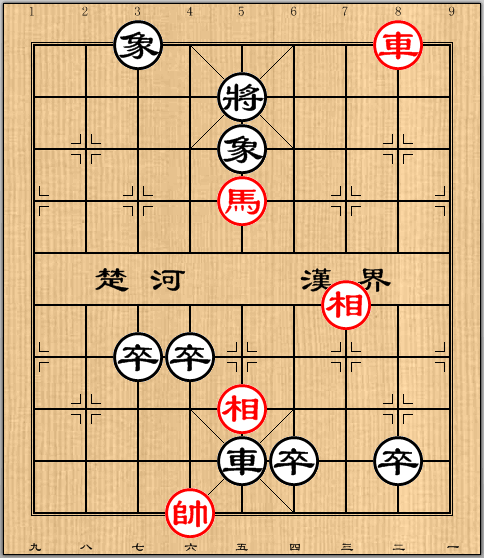
\includegraphics[width=5cm]{pic/天马行空例1.png}
\caption{天马行空例1}
\end{figure}

\begin{verbatim}
1. 车二平四,象5退7 [注1]
2. 马五进七,将5进1
3. 车四平三,将5平4 [注2]
4. 马七退六,将4退1 [注3]
5. 车三退一,将4退1
6. 马六进七,将4平5
7. 车三进一。

[注1]:红方伏有马五进七,将5平4,车四平六的杀棋。红方飞开中
象让出将路是唯一可以解杀的招法。另外此处选择车二平四而不是车
二平六,也至关重要,目的是避免让黑将在4路露头助攻的机会。试
讲车二平六的变化演变如下:车二平六、象5退7,马五进三、将5进1,
车六平七、将5平4,马三进四、车5平4!,帅六进一、卒4进1,帅六
退一、卒4进1,帅六平五、卒4平5,黑方抢杀在先。

[注2]:车四平三后伏有车三退二杀,黑方如将5平6,红方可以马七
进六入八角马位。

[注3]:构成天马行空杀型。
\end{verbatim}

\subsection{天马行空例2}
\label{sec-5-2-3}
\begin{figure}[H]
\centering
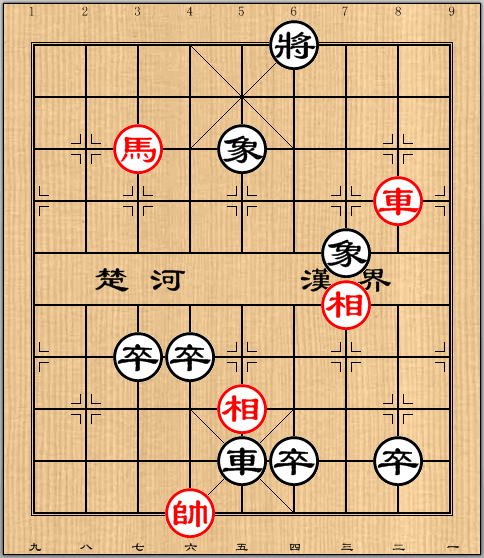
\includegraphics[width=5cm]{pic/天马行空例2.png}
\caption{天马行空例2}
\end{figure}

\begin{verbatim}
1. 车二进三,将6进1
2. 车二退一,将6退1 [注1]
3. 马七退五,将6平5 [注2]
4. 车二进一,将5进1
5. 车二平四,象5退7 [注3]
6. 马五进七,将5进1
7. 车四平二,将5平4 [注4]
8. 马三退四,将4退1
9. 车二退一,将4退1
10. 马四进三,将4平5
11. 车二进一。红胜。   
   
[注1]:如果将6进1,红方可以马七进六挂角。
[注2]:马七退五后伏有马五进三,将6平5,车二进一的杀棋。黑方
将6平5是唯一的选择。如果这一回合黑方走象5退7,红方可以车二平
五以花心车杀法取胜。
[注3]:此处车二平四而不是车二平六非常关键,目的是避免将来黑
将在4路肋道露头助攻的机会。试演变如下:车二平六,象5退3,马
五进三,将5进1,车六平七,将5平4,马三进四,车5平4!,帅六进
一,卒4进1,帅六退一,卒4进1,帅六平五,卒4平5,黑方反败为胜。
\end{verbatim}

\section{花心马-控制花心直接做杀}
\label{sec-5-3}

\subsection{花心马-控制花心直接做杀例1}
\label{sec-5-3-1}

\begin{figure}[H]
\centering
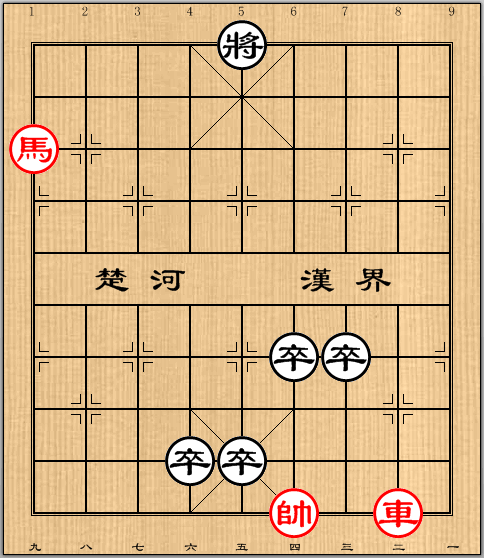
\includegraphics[width=5cm]{pic/花心马-控制花心直接做杀.png}
\caption{花心马-控制花心直接做杀例1}
\end{figure}


当黑方双士双象被剪除时,花心马对付光将的最基本的攻法就
是用花心马控制花心,然后用高车从纵横两路劈杀。下面介绍
两个由卧槽马变换为花心马做杀的例子。

\begin{verbatim}
1. 马九进七,将5平6 [注1]
2. 车二进四,将6进1   
3. 马七进五,将6平5 [注2]
4. 车二平五,将5平6
5. 马五退六,将6进1
6. 车五进四。花心车做杀,红胜。
   
[注1]:如果将5平4,那么红方可以车二进四,将4进1,马七退
六,下伏马六进八,将4平5,马八进七,走到低位花心马成杀,
黑方必须表态,黑方只能将4进1,红方还是可以马六进八继续
保持催杀,黑方将4平5,此时就可以使用前节介绍的停车问路
逼其表态的方法,用炮位马配合高车取胜。

[注2]: 红方马七进五,伏有马五退六,将6平5,马六进七,再
次走到低位花心马做杀的手段,黑方只能将6平5应对。
\end{verbatim}

\subsection{花心马-控制花心直接做杀例2}
\label{sec-5-3-2}
\begin{figure}[H]
\centering
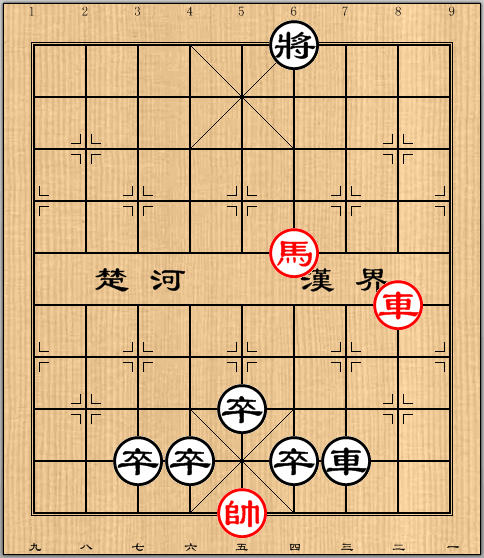
\includegraphics[width=5cm]{pic/花心马-控制花心直接做杀例2.png}
\caption{花心马-控制花心直接做杀例2}
\end{figure}

\begin{verbatim}
1. 马四进五,将6进1 [注1]
2. 马五进六,将6平5
3. 马六退七,将5平6
4. 车二平四。红胜。   
   
[注1]:黑方不走将6平5,是为了避免卧槽马配合高车的简易杀型。
\end{verbatim}


\section{花心马-前马后车}
\label{sec-5-4}
\begin{figure}[H]
\centering
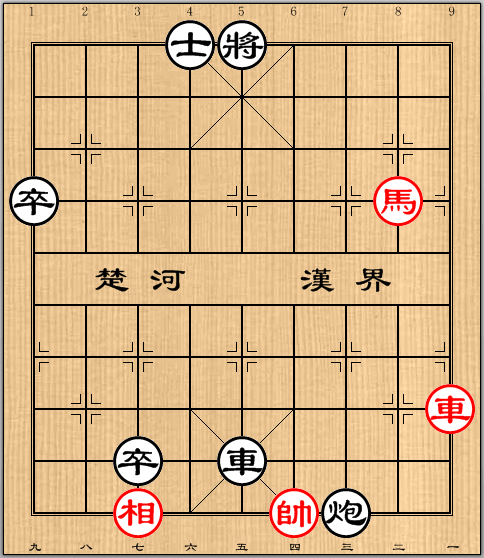
\includegraphics[width=5cm]{pic/花心马-前马后车.png}
\caption{花心马-前马后车}
\end{figure}

这个棋形可以先看一下车和马的位置,红方的车处于高位,纵向可以
打将,横向也可以打将,所以红方的车位置比较好,在红方车位好的
情况下,红马如果能走到花心马的位置,那么将对黑方产生很大的威
胁。

而这个棋形中红马是可以先手走到花心马的位置。
红方可以先马二进三卧槽将,黑方只能将5进1,红方再马三退四黑方
只能将5平6。黑方将5平6,表面上看是牵制住了红方的花心马,
但是红方如果走车一平四,那么黑方的这个将5平6就变成了先中后,
至此已经组成了杀形,绝杀无解了。

\begin{itemize}
\item 黑方如果置之不理,那么红方可以马四进三、将6平5,红方再车三
进六,黑方将5进1或者将5退1,红方再车四平六绝杀无解。值得一
提的是黑方如果置之不理,红方还有另外一路取胜的办法,那就是
马四退六、将6平5、马六进七,此时黑方如果上将或者下将那么红
方可以进车杀,如果黑方选择将5平4,那么红方可以选择平车杀。
\item 黑方如果走将6退1,那么红方可以走马四进六将,如果黑方走将6
进1,那么红方可以走马四退六将。
\end{itemize}


\section{花心马与其他马位的结合}
\label{sec-5-5}
\subsection{花心马-挂角将后回花心马位}
\label{sec-5-5-1}
\begin{figure}[H]
\centering
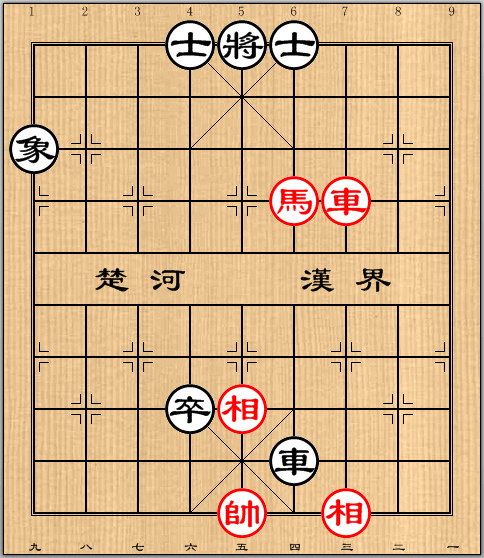
\includegraphics[width=5cm]{pic/花心马-挂角将后回花心马位.png}
\caption{花心马-挂角将后回花心马位}
\end{figure}

这一局中,红方的花心马可以先挂角将军,再车将,然后回到花心马
位做杀。从这一局可以体会下运马的技巧,有的时候并不是一味往前
冲杀,重回原位一样威力十足。另外从这一局还可以看到,当黑方有
底士自行阻挡黑将下将的通道时,是有利于花心马做杀的,黑方的4
路底士其实是红方的援军。

\begin{verbatim}
1. 马四进六,将5进1
2. 车三平五,将5平4
3. 马六退四,士4进5
4. 车五平六,红胜。
\end{verbatim}
\subsection{花心马-钓鱼马转低位花心马}
\label{sec-5-5-2}
\begin{figure}[H]
\centering
\includegraphics[width=5cm]{pic/花心马-钓鱼马转低位花心马.png}
\caption{花心马-钓鱼马转低位花心马}
\end{figure}

如图所示的局面,黑将的活动空间有限,红方可以施展“绕圈马”,
将马从钓鱼马位调整至低位红心马位做杀。

\begin{verbatim}
1. 马三退五,将6进1
2. 马五退三,将6退1
3. 马三进二,将6进1
4. 马二进三,将6退1
5. 车七平四。红胜。
\end{verbatim}
\subsection{花心马-钓鱼马转高位花心马}
\label{sec-5-5-3}
\begin{figure}[H]
\centering
\includegraphics[width=5cm]{pic/花心马-钓鱼马转高位花心马.png}
\caption{\label{hxm-dymzgwhxm}花心马-钓鱼马转高位花心马}
\end{figure}

通过这一局,大家可以再次体会一下,黑方的4路底士是如何“配合”红
方的高位花心马做杀的。

\begin{verbatim}
1. 马七退六,将4退1
2. 马六进四。红胜。
\end{verbatim}

值得一提的是,在图\ref{hxm-dymzgwhxm}所示的棋形中,即使没有黑方的4
路底士作为援军,红方依然有做杀的手段。参见下图

\begin{figure}[H]
\centering
\includegraphics[width=5cm]{pic/花心马-钓鱼马转高位花心马-黑无4路底士.png}
\caption{花心马-钓鱼马转高位花心马-黑无4路底士}
\end{figure}

红方取胜的招法如下:

\begin{verbatim}
1. 马七退六,将4退1
2. 马六进四,将4退1
3. 车三平六,将4平5
4. 车六平七,将5平4
5. 车七进五,将4进1
6. 车七退五,将4退1
7. 车七平六,将4平5
8. 车七平八,将5平4
9. 马四退六,将4进1
10. 车八进四,将4退1
11. 马六进七,将4平5
12. 车八进一。红胜。
\end{verbatim}




\chapter{其他的马位}
\label{sec-6}
\section{八角马-借帅力入角}
\label{sec-6-1}
\begin{figure}[H]
\centering
\includegraphics[width=5cm]{pic/借帅力入角.png}
\caption{借帅力入角}
\end{figure}

马二进四即可。
\section{象腰马转八角马}
\label{sec-6-2}
\begin{figure}[H]
\centering
\includegraphics[width=5cm]{pic/象腰马转八角马.png}
\caption{象腰马转八角马}
\end{figure}

象腰马同时具备向高钓马和八角马两个马位调整的可能性,可令对手
防不胜防。

\begin{verbatim}
1. 马二进四,士5退6
2. 车四平五,将5平6
3. 马四进六。红胜
\end{verbatim}


\section{象腰马转高钓马}
\label{sec-6-3}
\begin{figure}[H]
\centering
\includegraphics[width=5cm]{pic/象腰马转高钓马.png}
\caption{象腰马转高钓马}
\end{figure}

\begin{verbatim}
1. 车二进九,象5退7
2. 车二平三,将6进1
3. 兵四进一,将6进1
4. 车三平四,将6平5
5. 马六退七。红胜。
\end{verbatim}


\section{挂角马-前锋马-拔簧马}
\label{sec-6-4}
\begin{figure}[H]
\centering
\includegraphics[width=5cm]{pic/挂角马-前锋马-拔簧马.png}
\caption{挂角马-前锋马-拔簧马}
\end{figure}

\begin{verbatim}
1. 马八进六,将5进1
2. 车四进五,将5进1
3. 马六退五,士6进5
4. 车四退二,炮1平4
5. 车四平五,将5平4
6. 车五进二。
\end{verbatim}

\section{篡位马}
\label{sec-6-5}
\begin{figure}[H]
\centering
\includegraphics[width=5cm]{pic/篡位马.png}
\caption{篡位马}
\end{figure}

\begin{verbatim}
1. 马二退四,将5平6
2. 车四平三,将6平5
3. 车四平五,将5平6
4. 马四进六,士6进5
5. 车五平四,将6平5
6. 马六进五,将5平6
7. 车五平四,将6平5
8. 马五退三,将5平4
9. 车五平六,红胜。
\end{verbatim}

\section{中卒位马-象腰马-八角马}
\label{sec-6-6}
\begin{figure}[H]
\centering
\includegraphics[width=5cm]{pic/中卒位马-象腰马-八角马.png}
\caption{中卒位马-象腰马-八角马}
\end{figure}

\begin{verbatim}
1. 车二进九,将5进1
2. 马五进七,将5平6
3. 车二退五,将6退1
4. 车二平四,将6平5
5. 车四平五,将5平6
6. 马七退五,将6平5
7. 马五进四,将5平6
8. 马四退六,卒6平5
9. 帅五平四,卒4进1
10. 车五平四。红胜。
\end{verbatim}

\section{侧锋马-拔簧马}
\label{sec-6-7}
\begin{figure}[H]
\centering
\includegraphics[width=5cm]{pic/侧锋马-拔簧马.png}
\caption{侧锋马-拔簧马}
\end{figure}

红方马七进八,由高钓马转到侧锋马的位置上,黑方只能将4进1,
不能将4平5:
\begin{itemize}
\item 如果将4平5的话,那么红方的七路车可以进底线将军就完成绝杀了。
\item 如果黑方上将,红方可以车五进四,黑方上将或下将,红方都有车
七平五的杀棋。不过在这个棋形下,黑方的3路炮是个干扰项,红
方如果直接车七平五,黑方可以炮3退5垫,这样就延缓了红方的进
攻速度抢先做杀了。不过红方可以在车七平五之前先车七退五吃炮,
然后再车七进五,车七平五以拔簧马做杀。
\end{itemize}


\section{象腰马-钓鱼马-中卒马}
\label{sec-6-8}
\begin{figure}[H]
\centering
\includegraphics[width=5cm]{pic/象腰马-钓鱼马-中卒马.png}
\caption{象腰马-钓鱼马-中卒马}
\end{figure}


\begin{verbatim}
1. 马六退五,将6平5
2. 马五进七,将5平6
3. 车五平一,士6进5
4. 马七退五,将6退1
5. 车一进五。红胜。
\end{verbatim}


\section{中卒位马-钓鱼马-八角马-拔簧马}
\label{sec-6-9}
\begin{figure}[H]
\centering
\includegraphics[width=5cm]{pic/中卒位马-钓鱼马-八角马.png}
\caption{中卒位马-钓鱼马-八角马}
\end{figure}

红方中帅威力巨大,红方可以兵五进一,黑方只有将5进1吃,红方
再马五进七,黑方只有将5平6,红方再马七进六,黑方只能将6退1,
红方再车五进五将,黑方只能将6进1,红方再车五退三,拔簧马将,
黑方将6进1,红方再车五平四即可千里照面杀。



\chapter{综合杀法}
\label{sec-7}

\section{综合杀法-例1}
\label{sec-7-1}
\begin{figure}[H]
\centering
\includegraphics[width=5cm]{pic/综合杀法-例1.png}
\caption{综合杀法-例1}
\end{figure}

\begin{verbatim}
1. 车八进四,将4进1
2. 车八退一,将4退1
3. 马四退六,炮9退1 [注1]
4. 马六退八,炮9进1 [注2]
5. 马八进九,炮9退1 [注3]
6. 车八进一,将4进1
7. 马九进八,炮9进1 [注4]
8. 车八平七,炮9退2 [注5]
9. 马八退七,红胜。
   
[注1]:伏有钓鱼马杀。
[注2]:伏有侧面虎杀。
[注3]:又伏有钓鱼马杀。
[注4]:又伏有侧面虎杀。
[注5]:平车后又多了拔簧马的杀棋。
\end{verbatim}

\section{综合杀法-例2}
\label{sec-7-2}
\begin{figure}[H]
\centering
\includegraphics[width=5cm]{pic/综合杀法-例2.png}
\caption{综合杀法-例2}
\end{figure}

\begin{verbatim}
1. 马七退九,车7进4 [注1]
2. 帅四进一,车7退1
3. 帅四退一,车7平2
4. 车四退一,士4进5
5. 马九退七,将4退1 
6. 车四平五。[注2]

[注1]:马七退九后伏有马九进八,将4平5,马八退七,将5平4,车
四平六的杀棋。并且此时黑方难以解杀,黑车通过打将顿挫调动到2
路控制红马九进八的点位是最为顽强的应招,如改走士4进5,红方可
以马九退七,将4进1,车四退五,车7平4,仕四进五,车4退1,车四
平八,车4平3,车八平六杀。

[注2]:黑车虽然解了钓鱼马的杀棋,但是无法解除花心车的杀棋,
以下只能车换红马,红方胜定。
\end{verbatim}

\section{综合杀法-例3}
\label{sec-7-3}
\begin{figure}[H]
\centering
\includegraphics[width=5cm]{pic/综合杀法-例3.png}
\caption{综合杀法-例3}
\end{figure}

\begin{verbatim}
1. 车二平五,象3进5 [注1]
2. 马八退七,将5平4
3. 车五平六,象5进3 [注2]
4. 马六进四,将4平5
5. 车六进三,将5进1
6. 马四退五,士6进5
7. 车六退二,卒4平5
8. 车六平五,将5平4
9. 车六进二。红胜。

[注1]:本来红方可以直接马八退六,黑方只能将5平4,红方再走车
二平六就可以形成前马后车的棋形。可以将这个棋形和第3回合的棋
形进行比较,主要的区别是黑方多补了一手中象。此处红方让黑方多
补了一手中象可以加快进攻的速度,因为有中象时(参考第3回合的
阵型),红方伏有马六退八、将4平5、马八进七、将5退1、车六进四
的杀棋,黑方必须立刻应。而如果没有中象的话,黑方可以走一手卒
4平5,红方只能马六进四、将4平5、车六进三、将5进1、马四退五,
此时车7平6黑方就可以抢杀在先了。

[注2]:此处红方车五平六伏杀,黑方飞开中象是唯一的解招。可见
红方前面车二平五顿挫逼迫黑方飞中象之妙。
\end{verbatim}

\section{综合杀法-例4}
\label{sec-7-4}
\begin{figure}[H]
\centering
\includegraphics[width=5cm]{pic/综合杀法-例4.png}
\caption{综合杀法-例4}
\end{figure}

\begin{verbatim}
1. 马二退四,将5退1
2. 车三进四,将5进1
3. 车四平六,士6退5
4. 车六退五,将5平6
5. 车六平四。
\end{verbatim}
% Emacs 25.3.1 (Org mode 8.2.10)
\end{document}